% ******************************************************** %
%              TEMPLATE DE INFORME ORGA2 v0.1              %
% ******************************************************** %
% ******************************************************** %
%                                                          %
% ALGUNOS PAQUETES REQUERIDOS (EN UBUNTU):                 %
% ========================================
%                                                          %
% texlive-latex-base                                       %
% texlive-latex-recommended                                %
% texlive-fonts-recommended                                %
% texlive-latex-extra?                                     %
% texlive-lang-spanish (en ubuntu 13.10)                   %
% ******************************************************** %


\documentclass[a4paper]{article}
\usepackage[spanish]{babel}
\usepackage[utf8]{inputenc}
\usepackage{charter}   % tipografia
\usepackage{graphicx}
\usepackage{paralist} %itemize inline
\usepackage{underscore}
\usepackage{caratula}
\usepackage{url}
\usepackage[bottom]{footmisc}


% ********************************************************* %
% ~~~~~~~~              Code snippets             ~~~~~~~~~ %
% ********************************************************* %

\usepackage{color} % para snipets de codigo coloreados
\usepackage{fancybox}  % para el sbox de los snipets de codigo

\definecolor{litegrey}{gray}{0.94}

\newenvironment{codesnippet}{%
	\begin{Sbox}\begin{minipage}{\textwidth}\sffamily\small}%
	{\end{minipage}\end{Sbox}%
		\begin{center}%
		\vspace{-0.4cm}\colorbox{litegrey}{\TheSbox}\end{center}\vspace{0.3cm}}



% ********************************************************* %
% ~~~~~~~~         Formato de las páginas         ~~~~~~~~~ %
% ********************************************************* %

\usepackage{fancyhdr}
\pagestyle{fancy}
\renewcommand{\sectionmark}[1]{\markright{\thesection\ - #1}}

\fancyhf{}

\fancyhead[LO]{Sección \rightmark} % \thesection\ 
\fancyfoot[LO]{\small{María Carolina Gorosito, Muriel Picone Farías}}
\fancyfoot[RO]{\thepage}
\renewcommand{\headrulewidth}{0.5pt}
\renewcommand{\footrulewidth}{0.5pt}
\setlength{\hoffset}{-0.8in}
\setlength{\textwidth}{16cm}
\setlength{\headsep}{0.5cm}
\setlength{\textheight}{25cm}
\setlength{\voffset}{-0.7in}
\setlength{\headwidth}{\textwidth}
\setlength{\headheight}{13.1pt}

\renewcommand{\baselinestretch}{1.1}  % line spacing
\newcommand{\Mod}[1]{\ (\mathrm{mod}\ #1)}
% ******************************************************** %


\begin{document}


\thispagestyle{empty}
\materia{Organización del Computador II}
\submateria{Primer Cuatrimestre de 2020}
\titulo{Trabajo Práctico II}
\subtitulo{Implementación de filtros de imágenes con técnicas SIMD}
\integrante{María Carolina Gorosito}{293/18}{kaarogor@gmail.com}
\integrante{Muriel Picone Farías}{721/18}{muri.pic@gmail.com}

\maketitle
\newpage

\thispagestyle{empty}
\vfill
\begin{abstract}
Este trabajo tiene como objetivo examinar las ventajas de la utilización de instrucciones SIMD en el procesamiento de imágenes. Para ello, se implementaron en C y en Assembler tres filtros diferentes: \textit{Ocultar}, que convierte una imagen a escala de grises y la esconde en otra imagen; \textit{Descubrir}, que realiza la operación inversa, reconstruyendo la imagen oculta; y \textit{Zigzag}, que produce un efecto de zigzag desplazando píxeles y promediándolos con sus vecinos más cercanos. Se buscó implementar estos filtros de la manera más óptima posible pero atentendiendo a consideraciones de espacio (tamaño del código) y legibilidad, y preservando la funcionalidad y precisión de los filtros. Luego, en una segunda etapa, se realizaron modificaciones a las implementaciones con el fin de evaluar experimentalmente las variantes y sacar conclusiones sobre el efecto de las mismas sobre la performance.
\end{abstract}

\newpage
\thispagestyle{empty}
\vspace{3cm}
\tableofcontents

\newpage

\section{Introducción}

El objetivo de este trabajo práctico es implementar tres filtros de imágenes en Assembler utilizando técnicas de SIMD (Single Instruction, Multiple Data) para mejorar la performance de los algoritmos, aprovechando las herramientas que proveen los procesadores Intel para este tipo de implementaciones.
Los procesadores Intel tienen una arquitectura CISC (Complex Instruction Set Computer), por lo que cuentan con instrucciones que permiten realizar operaciones complejas. Entre estas instrucciones, se encuentran las instrucciones SIMD, en las extensiones SSE (Streaming SIMD Extensions) y AVX (Advanced Vector Extensions).
El modelo de procesamiento SIMD consiste en procesar múltiples datos en paralelo utilizando una única instrucción, frente al modelo SISD (Single Instruction, Single Data), en el que los datos se procesan de a uno, de manera secuencial. Esto hace que se puedan procesar varios píxeles de las imágenes en simultáneo, dando lugar a reducciones en el costo de procesamiento temporal de los filtros.
Además, la implementación de los filtros se acompañó con experimentos cuyos fines fueron evaluar el impacto de la utilización de este modelo de procesamiento en la performance temporal, analizar diferentes opciones de optimización y evaluar sobre bases empíricas algunas de las decisiones tomadas.

\section{Implementación}
A continuación se describe la implementación de cada uno de los filtros y se discuten las decisiones tomadas.

\subsection{Aspectos generales}
Los filtros procesan imagénes en formato BMP o mapa de bits. Este tipo de archivos posee un encabezado, que indica el formato, y píxeles. En el caso de las imágenes a color, los píxeles pueden ser de 24 o 32 bits, dependiendo de si tienen un componente de transparencia. Las componentes, de 8 bits cada una, se almacenan en memoria en el orden B (blue), G (green), R (red), A (alpha). Cada una es un entero sin signo que va de 0 a 255. En figura 1 se puede observar la estructura de un píxel ARGB (con la parte menos significativa a derecha).

\begin{figure}[!htb]
  \begin{center}
	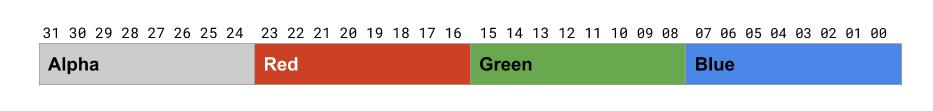
\includegraphics[scale=0.4]{img/RGB.jpg}
	\caption{Píxel ARGB}
  \end{center}
\end{figure}

Las imágenes en escala de grises, en cambio, tienen píxeles de un solo byte.
Considerando que cada registro {\tt xmm} es de 128 bits, cada uno puede contener 4 píxeles ARGB o 16 píxeles en escala de grises. \\
En cuanto al tamaño de las imágenes que procesan los filtros, deben tener un ancho mayor a 16 píxeles y múltiplo de 8 píxeles. Sin embargo, también se considerarán implementaciones alternativas que imponen restricciones adicionales; en particular, que el ancho sea múltiplo de 16 o de 32.
También es relevante señalar que los filtros \textit{Ocultar} y \textit{Descubrir} operan sobre dos imágenes, que deben tener las mismas dimensiones. 

\subsection{Ocultar}
El filtro \textit{Ocultar} consiste en convertir una imagen a escala de grises y luego ocultarla en otra, encriptándola mediante la operación {\tt xor} con los píxeles correspondientes de la imagen vista en espejo.
Dado que la utilización de instrucciones SIMD tiene como objetivo procesar datos en simultáneo para mejorar la performance, se decidió trabajar con la máxima cantidad de píxeles que no dieran lugar a casos borde, es decir, 8 píxeles por ciclo.
El filtro recibe como parámetros tres punteros: uno a la imagen a ocultar (en adelante {\tt src2}), otro a la imagen donde se va a ocultar la primera ({\tt src1}) y otro a la imagen destino ({\tt dst}). A estos punteros agregamos uno más al final de la imagen {\tt src1}, para levantar los píxeles de la imagen en espejo (en {\tt rax}).

\subsubsection{Ciclo}
Dado que no hay desfasajes de ningún tipo y son todas del mismo tamaño, las imágenes se recorren juntas. \\
En cada ciclo se realizan accesos a memoria en cuatro instancias: 1) para cargar píxeles de la imagen a ocultar, 2) para cargar píxeles de la imagen fuente en espejo, 3) para cargar píxeles de la imagen fuente, 4) para guardar los píxeles procesados en destino. En los casos 1 y 3 se levantan cuatro píxeles en un registro {\tt xmm}, se avanza el puntero esa misma cantidad de posiciones, y se levantan cuatro más. En el caso 2 se realiza el mismo procedimiento pero a la inversa, para levantar píxeles de la imagen en espejo. Finalmente, en el caso 4 se guardan los píxeles procesados en memoria. \\
Al final de cada ciclo, entonces, se modifican los punteros, incrementándose o decrementándose, según el caso en unidades equivalentes a 8 píxeles (es decir, 32). \\
Asimismo, se utiliza también un contador de píxeles procesados para poder determinar si se terminó de recorrer la imagen. Este se compara al inicio del ciclo\footnote{Si bien según la especificación provista por el enunciado el filtro no necesita funcionar con imágenes vacías, ubicar el ciclo al comienzo permite contemplar este caso adicional.} con el tamaño de la imagen en píxeles, y en caso de ser iguales, el ciclo termina. \\
Dado que los punteros iniciales están alineados a 16 bytes y todos los accesos respetan esa alineación, en todos los casos se utiliza la instrucción {\tt movdqa}.

\subsubsection{Conversión a escala de grises}
Dentro del ciclo, una vez levantados 8 píxeles de la imagen a ocultar, hay que convertirlos a escala de grises. Esta conversión se realiza con la siguiente fórmula: $(B + 2G + R)/4$. \\
Como hay que multiplicar solo la componente verde, es necesario separarlas. Para ello, se utiliza una máscara que luego se va shifteando a la izquierda, como se muestra en la figura 2.

\begin{figure}[h]
  \begin{center}
	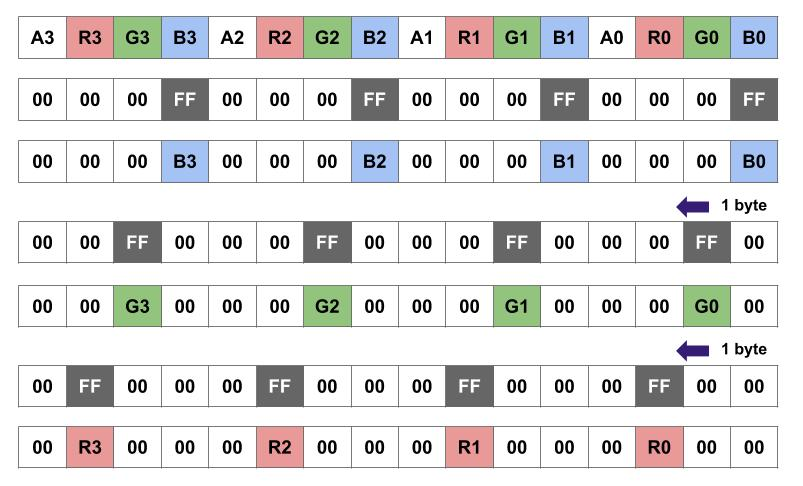
\includegraphics[scale=0.4]{img/ocultar/SepararComponentes.jpg}
	\caption{Separación de componentes RGB con una maścara}
  \end{center}
\end{figure}

En la figura 2 se muestran solo los primeros 4 píxeles. El procedimiento se repite para los segundos 4. \\
Una vez separados, se alinean las componentes G y R a derecha y se empaquetan los primeros 4 con los segundos 4 de cada componente con el fin de obtener words. Dado que hay que sumar componentes, trabajar con esta unidad en lugar de bytes permite mantener la precisión en caso de que la suma supere el valor 255, algo que es muy probable que ocurra. Este procedimiento se muestra en la figura 3.

\pagebreak

\begin{figure}[h]
  \begin{center}
	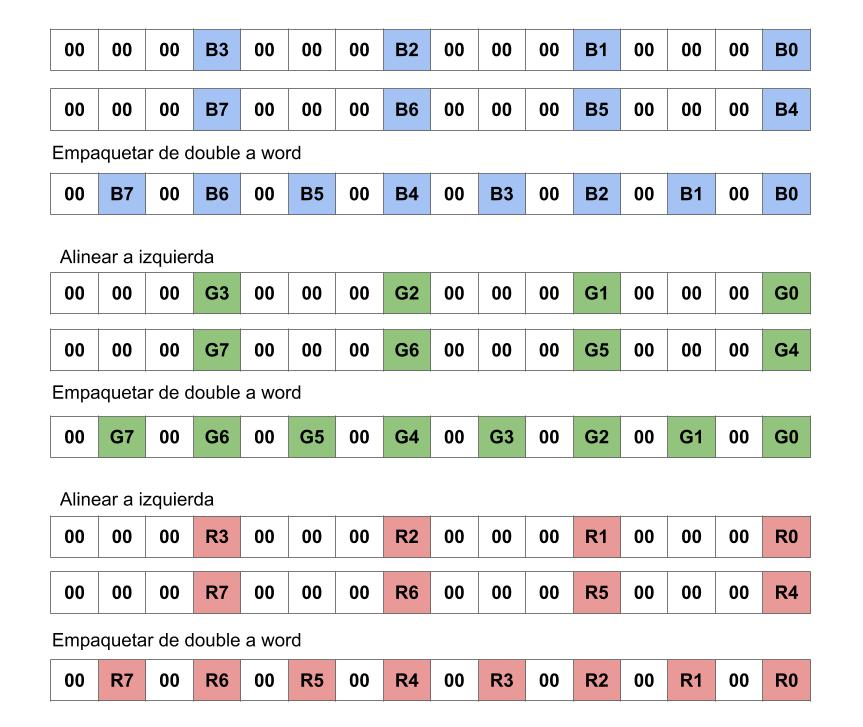
\includegraphics[scale=0.4]{img/ocultar/AlinearYEmpaquetar.jpg}
	\caption{Alineado a derecha y empaquetado de componentes RGB}
  \end{center}
\end{figure}

Luego, se multiplica G shifteando 1 bit a la izquierda y se suman las componentes verticalmente como indica la fórmula, con saturación para preservar lo más posible la imagen. Se divide el resultado por 4 shifteando 2 bits a derecha (figura 4).

\begin{figure}[h]
  \begin{center}
	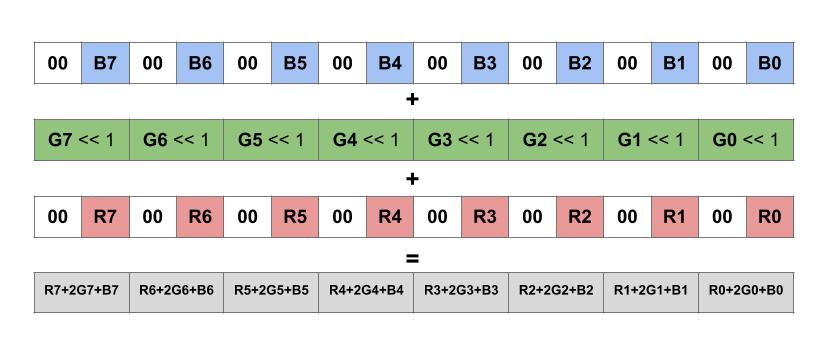
\includegraphics[scale=0.4]{img/ocultar/SumaVerticalGrayscale.jpg}
	\caption{Suma de componentes RGB}
  \end{center}
\end{figure}

Finalmente, se empaquetan los dos píxeles en escala de grises resultantes a su tamaño final, es decir, de un byte. Los resultados quedan en un registro {\tt xmm} como se muestra en la figura 5.

\begin{figure}[h]
  \begin{center}
	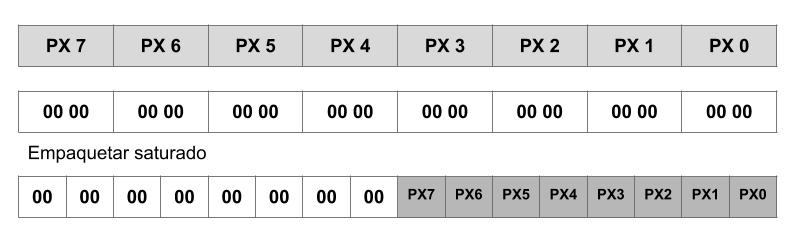
\includegraphics[scale=0.4]{img/ocultar/EmpaquetarSaturadoGrayscale.jpg}
	\caption{Empaquetado con saturación de píxeles en escala de grises}
  \end{center}
\end{figure}

\pagebreak

\subsubsection{Reorganización de bits y encriptación con {\tt xor}}
De los 8 bits de los píxeles en escala de grises, solo se van a ocultar los 6 más significativos, 2 en las posiciones menos significativas de cada componente de color de la imagen destino. Antes de guardarlos en {\tt dst}, estos bits se encriptan realizando una operación de {\tt xor} con los bits 2 y 3 de {\tt src1} pero del píxel correspondiente a la imagen vista en espejo. \\
En primer lugar, se separan los bits del píxel en escala de grises y se reorganizan en los pares de bits que luego se guardaran en cada componente.
Este procedimiento se realiza para los 6 bits a guardar. En el caso de la componente azul, es necesario obtener los bits 7 y 4, en ese orden. Para ello, con una máscara y la instrucción {\tt pand} se filtra el bit 7 y se desplaza hacia la posición menos significativa. Luego, se modifica la máscara desplazándola para obtener el bit 4, que se filtra en otro registro y se ubica en la posición 1 del byte resultante. Finalmente se combinan los registros que contienen los bits 7 y 4 con {\tt por}. Estos pasos se muestran en la figura 6 (se muestran solo 4 píxeles a modo de ejemplo).

\begin{figure}[!htb]
  \begin{center}
	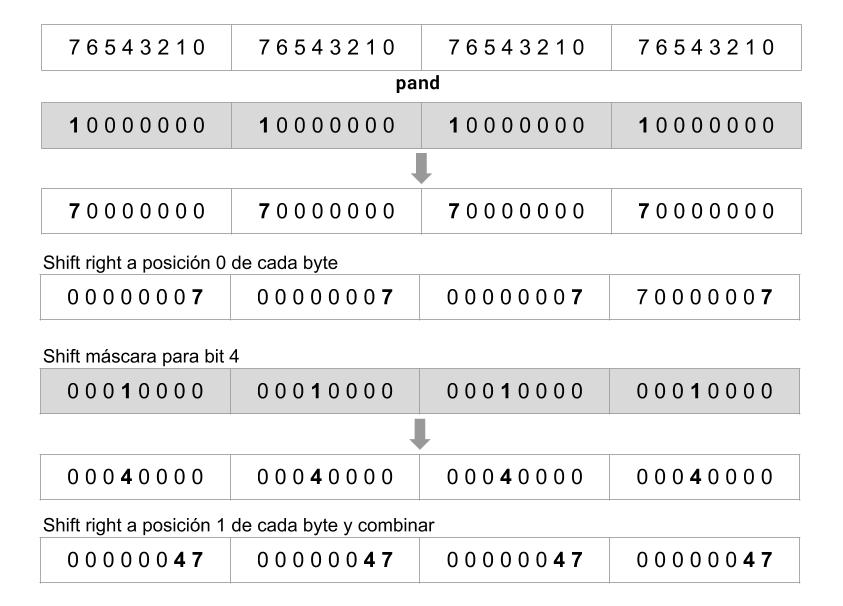
\includegraphics[scale=0.4]{img/ocultar/ReorganizarBits.jpg}
	\caption{Separación y combinación de bits 4 y 7 (a ocultar en componente B)}
  \end{center}
\end{figure}

El procedimiento para los bits correspondientes a las componentes verde y roja es igual, con las modificaciones necesarias de las posiciones a shiftear en cada caso. \\
Una vez separados los pares de bits, utilizando operaciones de desempaquetado se combinan los bits que van a ir en las componentes G y B, por un lado, y R con un registro de ceros, por el otro. Luego, se combinan los resultados de estas operaciones con un nuevo desempaquetado para obtener el resultado de la figura 7.

\pagebreak

\begin{figure}[h]
  \begin{center}
	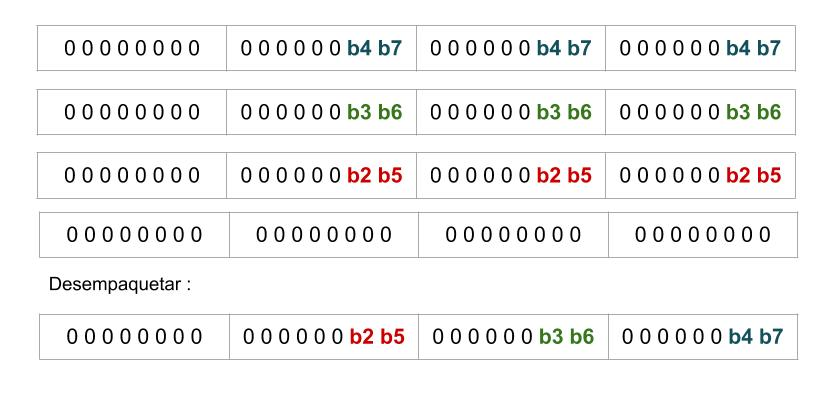
\includegraphics[scale=0.4]{img/ocultar/DesempaquetarParesDeBits.jpg}
	\caption{Combinación de bits para guardar en RGB}
  \end{center}
\end{figure}

Para la encriptación, se traen de memoria los últimos 4 píxeles de la imagen. Los píxeles se cargan en orden; por esta razón, para utilizarlos en espejo es necesario invertirlos. Usando {\tt pshufd} se reorganizan como se muestra en la figura 8.

\begin{figure}[!htb]
  \begin{center}
	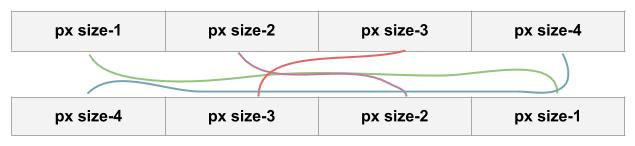
\includegraphics[scale=0.4]{img/ocultar/PixelShuffle.jpg}
	\caption{Shuffle de píxeles de imagen en espejo}
  \end{center}
\end{figure}

Luego, se ponen los bits 2 y 3 en las posiciones menos significativas mediante shifts, se filtran con una máscara, y se realiza el {\tt xor} con los bits que se van a guardar.

\subsubsection{Combinación con {\tt src1}}
Finalmente, se cargan desde memoria los 8 píxeles de {\tt src1} donde se van a ocultar los bits encriptados. Con una máscara se ponen en blanco los últimos dos bits de estos píxeles, luego se combinan con los bits encriptados usando {\tt por} y se guardan en {\tt dst}.


\subsection{Descubrir}
El filtro \textit{Descubrir} es complementario de \textit{Ocultar} y consiste en reconstruir la imagen ocultada. La imagen destino será una imagen en escala de grises, ya que sus componentes R, G y B contendrán el mismo píxel en escala de grises ocultado previamente. Como al ocultar la imagen no se habían conservado los últimos dos bits, estos quedarán en cero. \\
Recibe como parámetro dos punteros, uno a la imagen fuente (en adelante, {\tt src}) y otra a la imagen destino (en adelante {\tt dst}). Al igual que en \textit{Ocultar}, a estos punteros agregamos uno al final para levantar los píxeles de la imagen en espejo (también en {\tt rax}). En este caso también se procesan de a 8 píxeles por ciclo para aprovechar todo lo posible el espacio en los registros {\tt xmm} pero evitando casos borde.

\subsubsection{Ciclo}
Dadas sus similitudes con \textit{Ocultar}, el ciclo es análogo. Se realizan 3 accesos a memoria, para levantar 8 píxeles de la imagen fuente, de la imagen fuente en espejo y guardar el resultado en destino, respectivamente. También aquí las posiciones están alineadas, por lo que en todos los casos se utiliza {\tt movdqa}.

\subsubsection{Desencriptación}
El proceso comienza cargando 8 píxeles de memoria y extrayendo los bits encriptados de la imagen a reconstruir, es decir, los dos menos significativos de las componentes R, G y B, con un máscara. De este proceso se obtienen los bits que se muestran en la figura 9 (solo se muestran los de un píxel a modo de ejemplo). Debajo puede verse el bit reconstruido.

\begin{figure}[!htb]
  \begin{center}
	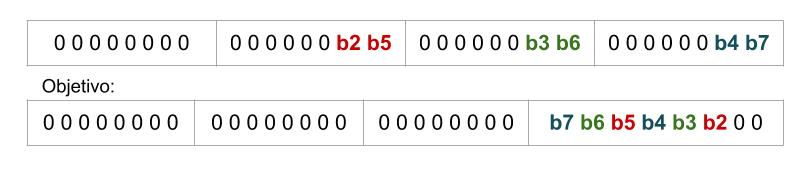
\includegraphics[scale=0.4]{img/descubrir/PixelGSReconstruido.jpg}
	\caption{Píxel reconstruido}
  \end{center}
\end{figure}

Sin embargo, es conveniente desencriptarlo antes de reconstruirlo. Para ello, se cargan los últimos 8 píxeles de la imagen en espejo con el puntero mencionado más arriba y se reordenan con el mismo procedimiento utilizado en el filtro anterior. Con una máscara, se filtran los bits 2 y 3, luego se desplazan hacia las posiciones menos significativas mediante {\tt shift} y finalmente se realiza el {\tt xor} entre los píxeles de la imagen oculta y los obtenidos en este paso.

\subsubsection{Reconstrucción del píxel}
Como es necesario reordenar bits, no se pueden utilizar operaciones de shuffle ya que no hay instrucciones de este tipo disponible para unidades tan pequeñas. Por este motivo, el procedimiento se realiza con máscaras y operaciones de shift. \\
Se trabaja con una única máscara que se va shifteando para obtener el bit correspondiente. A continuación se detalla el procedimiento para los bits 2 y 3 (es análogo para los siguientes).

\begin{figure}[!htb]
  \begin{center}
	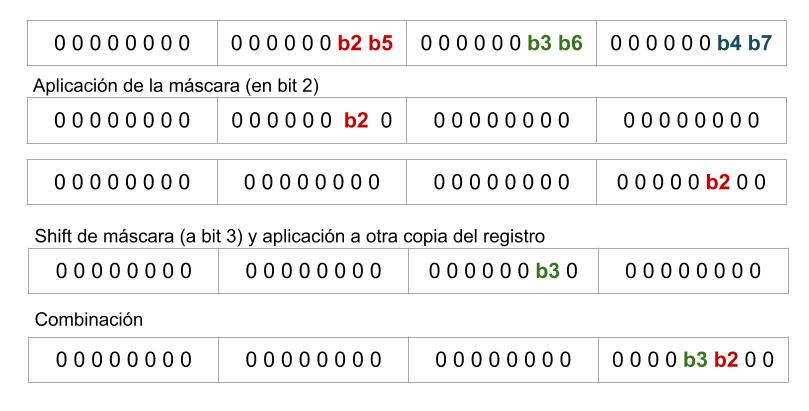
\includegraphics[scale=0.4]{img/descubrir/ReconstruccionPx.jpg}
	\caption{Reconstrucción del píxel (bits 2 y 3)}
  \end{center}
\end{figure}

Como se puede ver en la figura 10, primero se carga una máscara que filtra los bits 2. Se realiza una copia del registro original, se aplica la máscara y se desplazan los bits 2 a su posición correspondiente. Este registro será el acumulador, es decir, a medida que se vayan aislando y reubicando los bits siguientes se irán combinando con este. Es lo que ocurre con el bit 3: se shiftea la máscara utilizada para los bits 2 las posiciones necesarias, se filtra una nueva copia del registro original de manera tal que queden solo los bits 3 y se combina con el acumulador.

\subsubsection{Copia en las tres componentes}
Finalmente, resta copiar el píxel reconstruido en las tres componentes y rellenar la componente A con {\tt FF} (ver imagen abajo). La copia se realiza mediante una operación de shuffle, que deja en cero la parte de la componente A para luego completarla combinándola con una máscara (figura 11). Los 8 píxeles resultantes se guardan en destino.

\begin{figure}[!htb]
  \begin{center}
	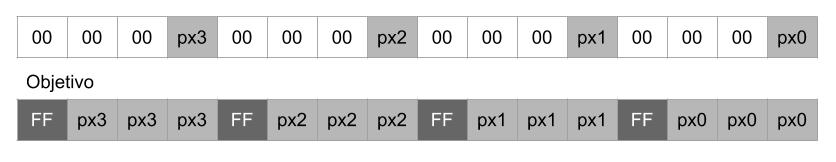
\includegraphics[scale=0.4]{img/descubrir/GrisesPor3.jpg}
	\caption{Armado de los píxeles finales}
  \end{center}
\end{figure}

\subsection{Zigzag}
El filtro \textit{Zigzag} consiste en generar un efecto de zig zag en la imagen desplazando 2 píxeles las filas impares (en direcciones opuestas) y realizando un promedio de cada píxel con sus cuatro vecinos más cercanos en las filas pares. Además, debe agregarse a la imagen un marco blanco de dos píxeles. \\
En este caso, si bien la imagen también cumple la condición de ser múltiplo de 8, la cantidad de píxeles procesados simultáneamente (si solo se consideran los que efectivamente van a guardarse en memoria) es de 4. Esta decisión se debió a que en las filas pares para procesar un píxel es necesario contar con los dos píxeles que están a su derecha y los dos de su izquierda. Así, si se levantan de memoria los píxeles del 0 al 7, solo se podrán procesar los del 2 al 5.

\subsubsection{Ciclo}
El filtro recibe como parámetros un puntero a la imagen fuente y otro a la imagen destino. \\
Cuenta con una sección llamada $\tt{distribuidorFilas}$. Luego de terminar de recorrer una fila, se salta aquí para avanzar el contador de filas, ver si ya se terminó de recorrer la imagen, calcular los punteros al inicio de la próxima fila y decidir si se trata de una fila par, 1 o 3. Si bien los saltos podrían afectar negativamente la performance, se optó por agrupar todas estas operaciones en una única sección con el objetivo de evitar la repetición de código y mejorar la legibilidad, y reservar las posibles optimizaciones para la etapa de experimentación.

\subsubsection{Marco blanco}
Para evitar tener que recorrer la imagen por columnas para poner el marco en los laterales, se decidió ir agregándolo a medida que se procesaba toda la imagen. Además, de esta forma se resolvían inmediatamente los casos borde en los que los píxeles no podían procesarse por no tener vecinos. \\
El filtro comienza completando las dos primeras filas con blanco en la sección $\tt{filasBlancas}$, para luego llegar al distribuidor de filas. El distribuidor de filas también analiza si ya se llegó a la fila $\tt{width-2}$, es decir, la fila en la que comienza el marco inferior, y salta a la sección $\tt{filasBlancas}$ nuevamente.

\subsubsection{Filas impares}
En las filas impares no es necesario realizar ningún procesamiento sobre los píxeles sino simplemente levantarlos de memoria y almacenarlos en la posición desplazada en la imagen destino. Para poder hacer esto, estas filas se recorren con los punteros a fuente y destino desplazados en dos píxeles, es decir, en 8 bytes.

\subsubsection{Filas pares}
En las filas impares hay que calcular el promedio de la suma por componentes del píxel a procesar y sus cuatro vecinos más cercanos, es decir que para cada píxel es necesario contar con dos vecinos a izquierda y dos a derecha para poder procesarlo. Por este motivo, se trabaja con 8 píxeles de la imagen fuente para obtener 4 de la imagen destino. \\
Los primeros 4 píxeles se levantan fuera del ciclo, ya que en cada iteración se trabaja con 4 píxeles levantados en el ciclo anterior y 4 nuevos. Esto permite evitar acceder a memoria para levantar datos ya levantados previamente. \\
Ya dentro del ciclo, en la primera iteración se cuenta con los píxeles 0 a 3 en un registro y se levantan los píxeles 4:7 de {\tt src}.
A continuación, se realizan copias de los registros y se van desplazando un píxel a derecha hasta tener 5 registros con los píxeles escalonados, como se muestra en la figura 12.

\begin{figure}[!htb]
  \begin{center}
	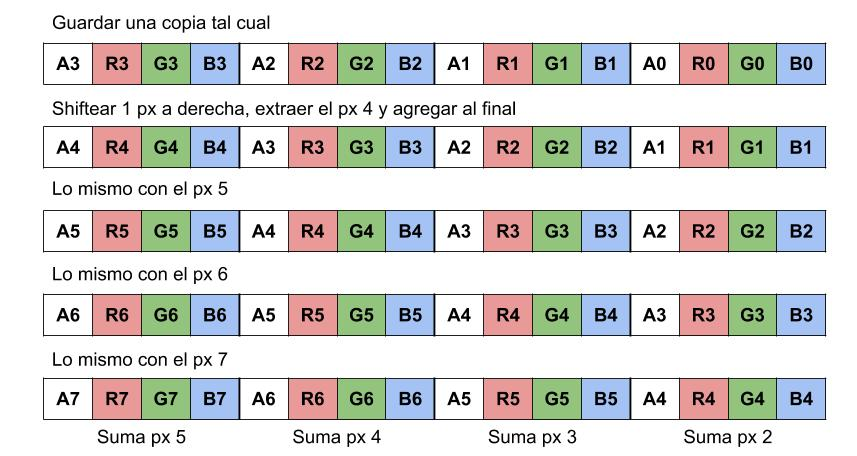
\includegraphics[scale=0.4]{img/zigzag/FilasPares1.jpg}
	\caption{Copia y shifteo de registros}
  \end{center}
\end{figure}

Esto permite tener en la primera columna (de derecha a izquierda) los 5 píxeles que hay que sumar para el píxel 2 de la imagen destino\footnote{En este punto es importante recordar que los píxeles 0 y 1 no se pueden procesar por no tener vecinos y además en la imagen destino corresponderán al marco.}, en la segunda los que se necesitan para el píxel 3, y así sucesivamente. \\
De esta forma, se puede obtener la suma componente a componente realizando sumas verticales, pero antes es necesario desempaquetar los bytes a words para no perder precisión al realizarla. Al desempaquetar, los registros se dividen en parte alta y parte baja y quedan como se muestra en la figura 13.

\begin{figure}[h]
  \begin{center}
	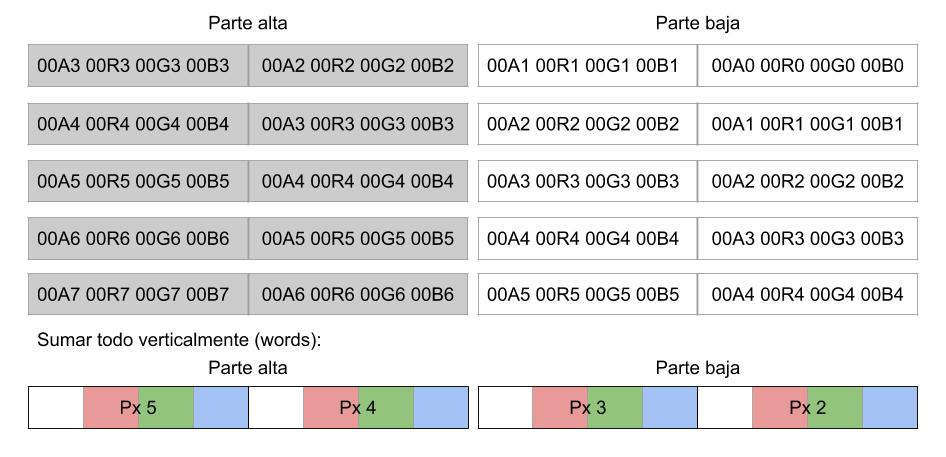
\includegraphics[scale=0.3]{img/zigzag/FilasPares2.jpg}
	\caption{Desempaquetar byte a word}
  \end{center}
\end{figure}

\pagebreak

Del procedimiento anterior se obtienen dos registros con las sumas de cada píxel y sus cuatro vecinos requeridos. El paso siguiente es hacer la división para calcular el promedio, pero dado que la división debe hacerse por 5, es necesario convertir los datos a float single precision. Para ello, se desempaquetan esos dos registros para obtener 4 con datos de 32 bits (figura 14), y luego se realizan la conversión y la división.

\begin{figure}[!htb]
  \begin{center}
	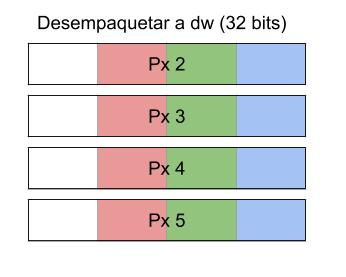
\includegraphics[scale=0.4]{img/zigzag/FilasPares3.jpg}
	\caption{Desempaquetado a 32 bits}
  \end{center}
\end{figure}

Finalmente, para poder guardar los píxeles en memoria, es necesario volver a convertirlos a enteros y al tamaño correspondiente. Con este fin, se realiza la conversión y luego se hace un empaquetado con saturación de double word a word. Después, se vuelve a realizar una operación de empaquetado para obtener un solo registro con los 4 píxeles a guardar en destino (figura 15).

\begin{figure}[!htb]
  \begin{center}
	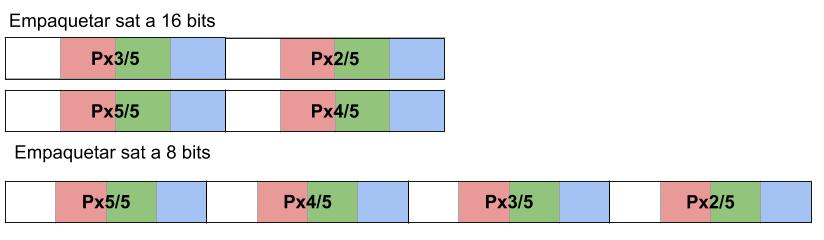
\includegraphics[scale=0.4]{img/zigzag/FilasPares4.jpg}
	\caption{Empaquetado a byte}
  \end{center}
\end{figure}


\section{Experimentación}

Con el objetivo de evaluar las decisiones tomadas, identificar qué partes o aspectos de las implementaciones pueden ser optimizados y analizar posibles mejoras en su rendimiento, se realizaron los experimentos que se detallan a continuación.

\subsection{Metodología}
Para analizar el rendimiento de las implementaciones se midieron los tiempos de ejecución. Esta medición se realizó con la instrucción de Assembler {\tt rdtsc}, que permite obtener el valor del \textit{Time Stamp Counter} (TSC) del procesador. Así, se obtiene la diferencia entre los contadores antes y después de la llamada a la función, es decir, la cantidad de ciclos de esa ejecución. \\
Dado que este registro es global al procesado, puede haber factores externos que afecten esta medición. Por este motivo, todos los experimentos fueron ejecutados con la menor cantidad posible de procesos corriendo en segundo plano. \\
Ademas, con el fin de eliminar el ruido en las mediciones, se realizaron 1000 ejecuciones para cada condición a evaluar. Estas ejecuciones y el almacenamiento de los resultados se automatizaron con un script en Python que guarda el valor para cada ejecución. Contar con los datos individuales en lugar de trabajar directamente con el promedio de las mediciones permite la eliminación de outliers; consideramos como tales a los valores que están a más de 3 desviaciones estándar de la media. En los gráficos se reportan la media de los ciclos de clock y el desvío estándar para cada implementación. \\
Las mediciones fueron realizadas en una computadora con un procesador Intel Core i5-4200U CPU @ 1.60GHz, con 8 GB de RAM y Ubuntu 18.04.

\subsection{Análisis de costo de procesamiento}
Los tres filtros pueden dividirse en tres partes claramente diferenciadas, asociadas con distintos tipos de operaciones: hay instrucciones dedicadas a recorrer la imagen (es decir, las correspondientes al ciclo), otras cuya función es leer y escribir información en memoria y, finalmente, otras encargadas de procesar los píxeles levantados de memoria. Dependiendo de las características de cada filtro, estas tres partes tendrán diferentes costos relativos. Por ejemplo, es posible que en un filtro la mayor parte de los ciclos de clock estén destinados al procesamiento de los píxeles mientras que en otro los accesos a memoria tengan el mayor costo. \\
Esta información puede resultar muy útil para orientar el proceso de elección de optimizaciones, dado que es más probable que estas tengan un efecto más significativo si afectan a aquellos aspectos que tienen un mayor peso en el costo total. Con este fin, se hicieron dos versiones parciales de los filtros: una en la que solo se conservó el recorrido de la imagen y otra en la que se recorre la imagen y se lee y escribe en memoria. Al analizar los resultados obtenidos de estas versiones junto con las versiones originales se obtuvo el costo relativo de cada parte.

\begin{figure}[h]       
    \fbox{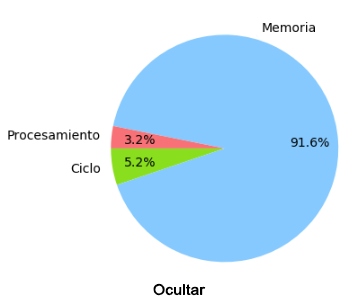
\includegraphics[scale=0.5]{img/partesOcultarnew.png}}   
    \hspace{10px}
    \fbox{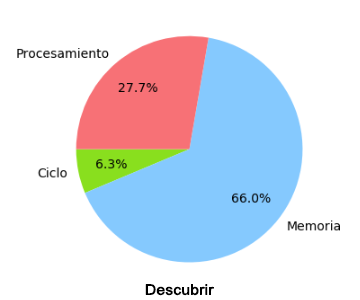
\includegraphics[scale=0.5]{img/partesDescubrirnew.png}}
    \hspace{10px}
    \fbox{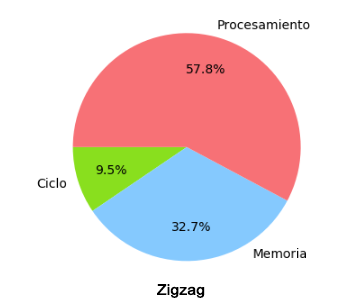
\includegraphics[scale=0.5]{img/partesZigzagnew.png}}
    \caption{Costo relativo de los accesos a memoria, ciclo y procesamiento de los píxeles en los tres filtros}
\end{figure}

Como se puede observar en la figura 16, los tres filtros presentan perfiles diferentes. En \textit{Ocultar} el costo de los accesos a memoria representa casi la totalidad del ciclo, mientras que en \textit{Descubrir} representa aproximadamente dos tercios y en \textit{Zigzag} solo uno. El costo del ciclo es relativamente pequeño en todos los casos aunque, previsiblemente, es algo más alto en \textit{Zigzag} debido a la inclusión del distribuidor de filas, pero aun así no supera el 10\%. El costo asociado al procesamiento también es muy variable: en \textit{Ocultar} apenas supera el 3\%, mientras que en \textit{Descubrir} casi alcanza el 30\% y en \textit{Zigzag} está cerca del 60\%.
\\ En línea con esto, es probable que \textit{Ocultar} obtenga mayores beneficios de optimizaciones en los accesos a memoria, mientras que en \textit{Zigzag} probablemente se vean mayores efectos en las optimizaciones del procesamiento. En \textit{Descubrir}, si bien la memoria también tiene el mayor costo, en este caso se encuentra más balanceado con el procesamiento y por eso quizás se obtengan mejores resultados combinando distintas estrategias.

\subsection{Experimento 0: Comparación C vs ASM}
\subsubsection{Descripción del problema}
Un primer paso en la evaluación de optimizaciones de rendimiento es analizar el punto de partida de los filtros en Assembler en comparación con los mismos algoritmos implementados en C. Para ello, se realizó un experimento que analiza las diferencias entre la implementación en Assembler con la implementación en C utilizando distintos flags del compilador. Los filtros en C fueron compilados utilizando los flags que se detallan a continuación:

\begin{itemize}
\item O$\textsubscript{0}$: opción default. Reduce levemente el tiempo de compilación y el uso de la memoria, aumentando levemente el tiempo de ejecución y el tamaño del código.
\item O$\textsubscript{1}$: empeora el tiempo de compilación y el uso de memoria, pero se reduce el tiempo de ejecución y el tamaño del código.
\item O$\textsubscript{2}$: mejora bastante el tiempo de ejecución, a costa de uso de memoria y tiempo de compilación.
\item O$\textsubscript{3}$: una optimización a lo indicado en O2: el tiempo de ejecución disminuye aún más, pero empeora bastante el tiempo de compilación.
\item O$\textsubscript{s}$: reduce el tamaño del código a costa de tardar más en la compilación.
\item O$\textsubscript{fast}$: lo mismo que O3, pero habilitando algunas optimizaciones que no cumplen algunos estándares, por lo que debe usarse con cautela.
\end{itemize}

\begin{figure}[!htb]
  \begin{center}
	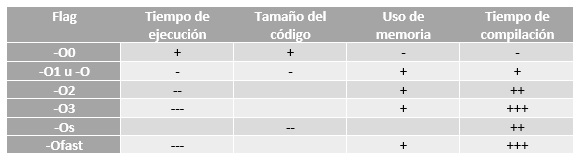
\includegraphics[scale=0.7]{img/flags.jpg}
	\caption{Resumen del funcionamiento de los flags}
  \end{center}
\end{figure}

Vale la pena notar que los flags O$\textsubscript{3}$ y O$\textsubscript{fast}$ pueden causar que el programa requiera mayor espacio en la pila en el tiempo de ejecución.

\subsubsection{Hipótesis}
La implementación en assembler, gracias a la utilización de instrucciones SIMD, debería tener una mejor performance que la implementación en C, independientemente del flag de optimización utilizado.

\subsubsection{Resultados}
Tal como se esperaba, la implementación en Assembler tiene un mejor desempeño que todas las versiones de C en los tres casos.
En el caso de \textit{Ocultar}, la versión en assembler es un 70.38\% más rápida que la mejor implementación de C, que en este caso es cO$\textsubscript{2}$. La media para assembler fue de 1362708 ciclos, con un desvío estándar de 116263, mientras que la media para cO$\textsubscript{2}$ fue de 4600875, con un desvío de 122723. En la figura 18 se puede ver la comparación entre el rendimiento de las distintas condiciones. Llamativamente, las versiones cO$\textsubscript{fast}$ y cO$\textsubscript{3}$ tuvieron un rendimiento más bajo que cO$\textsubscript{2}$. cO$\textsubscript{s}$ y cO$\textsubscript{0}$, previsiblemente, tuvieron los peores rendimientos.

\begin{figure}[!htb]
  \begin{center}
	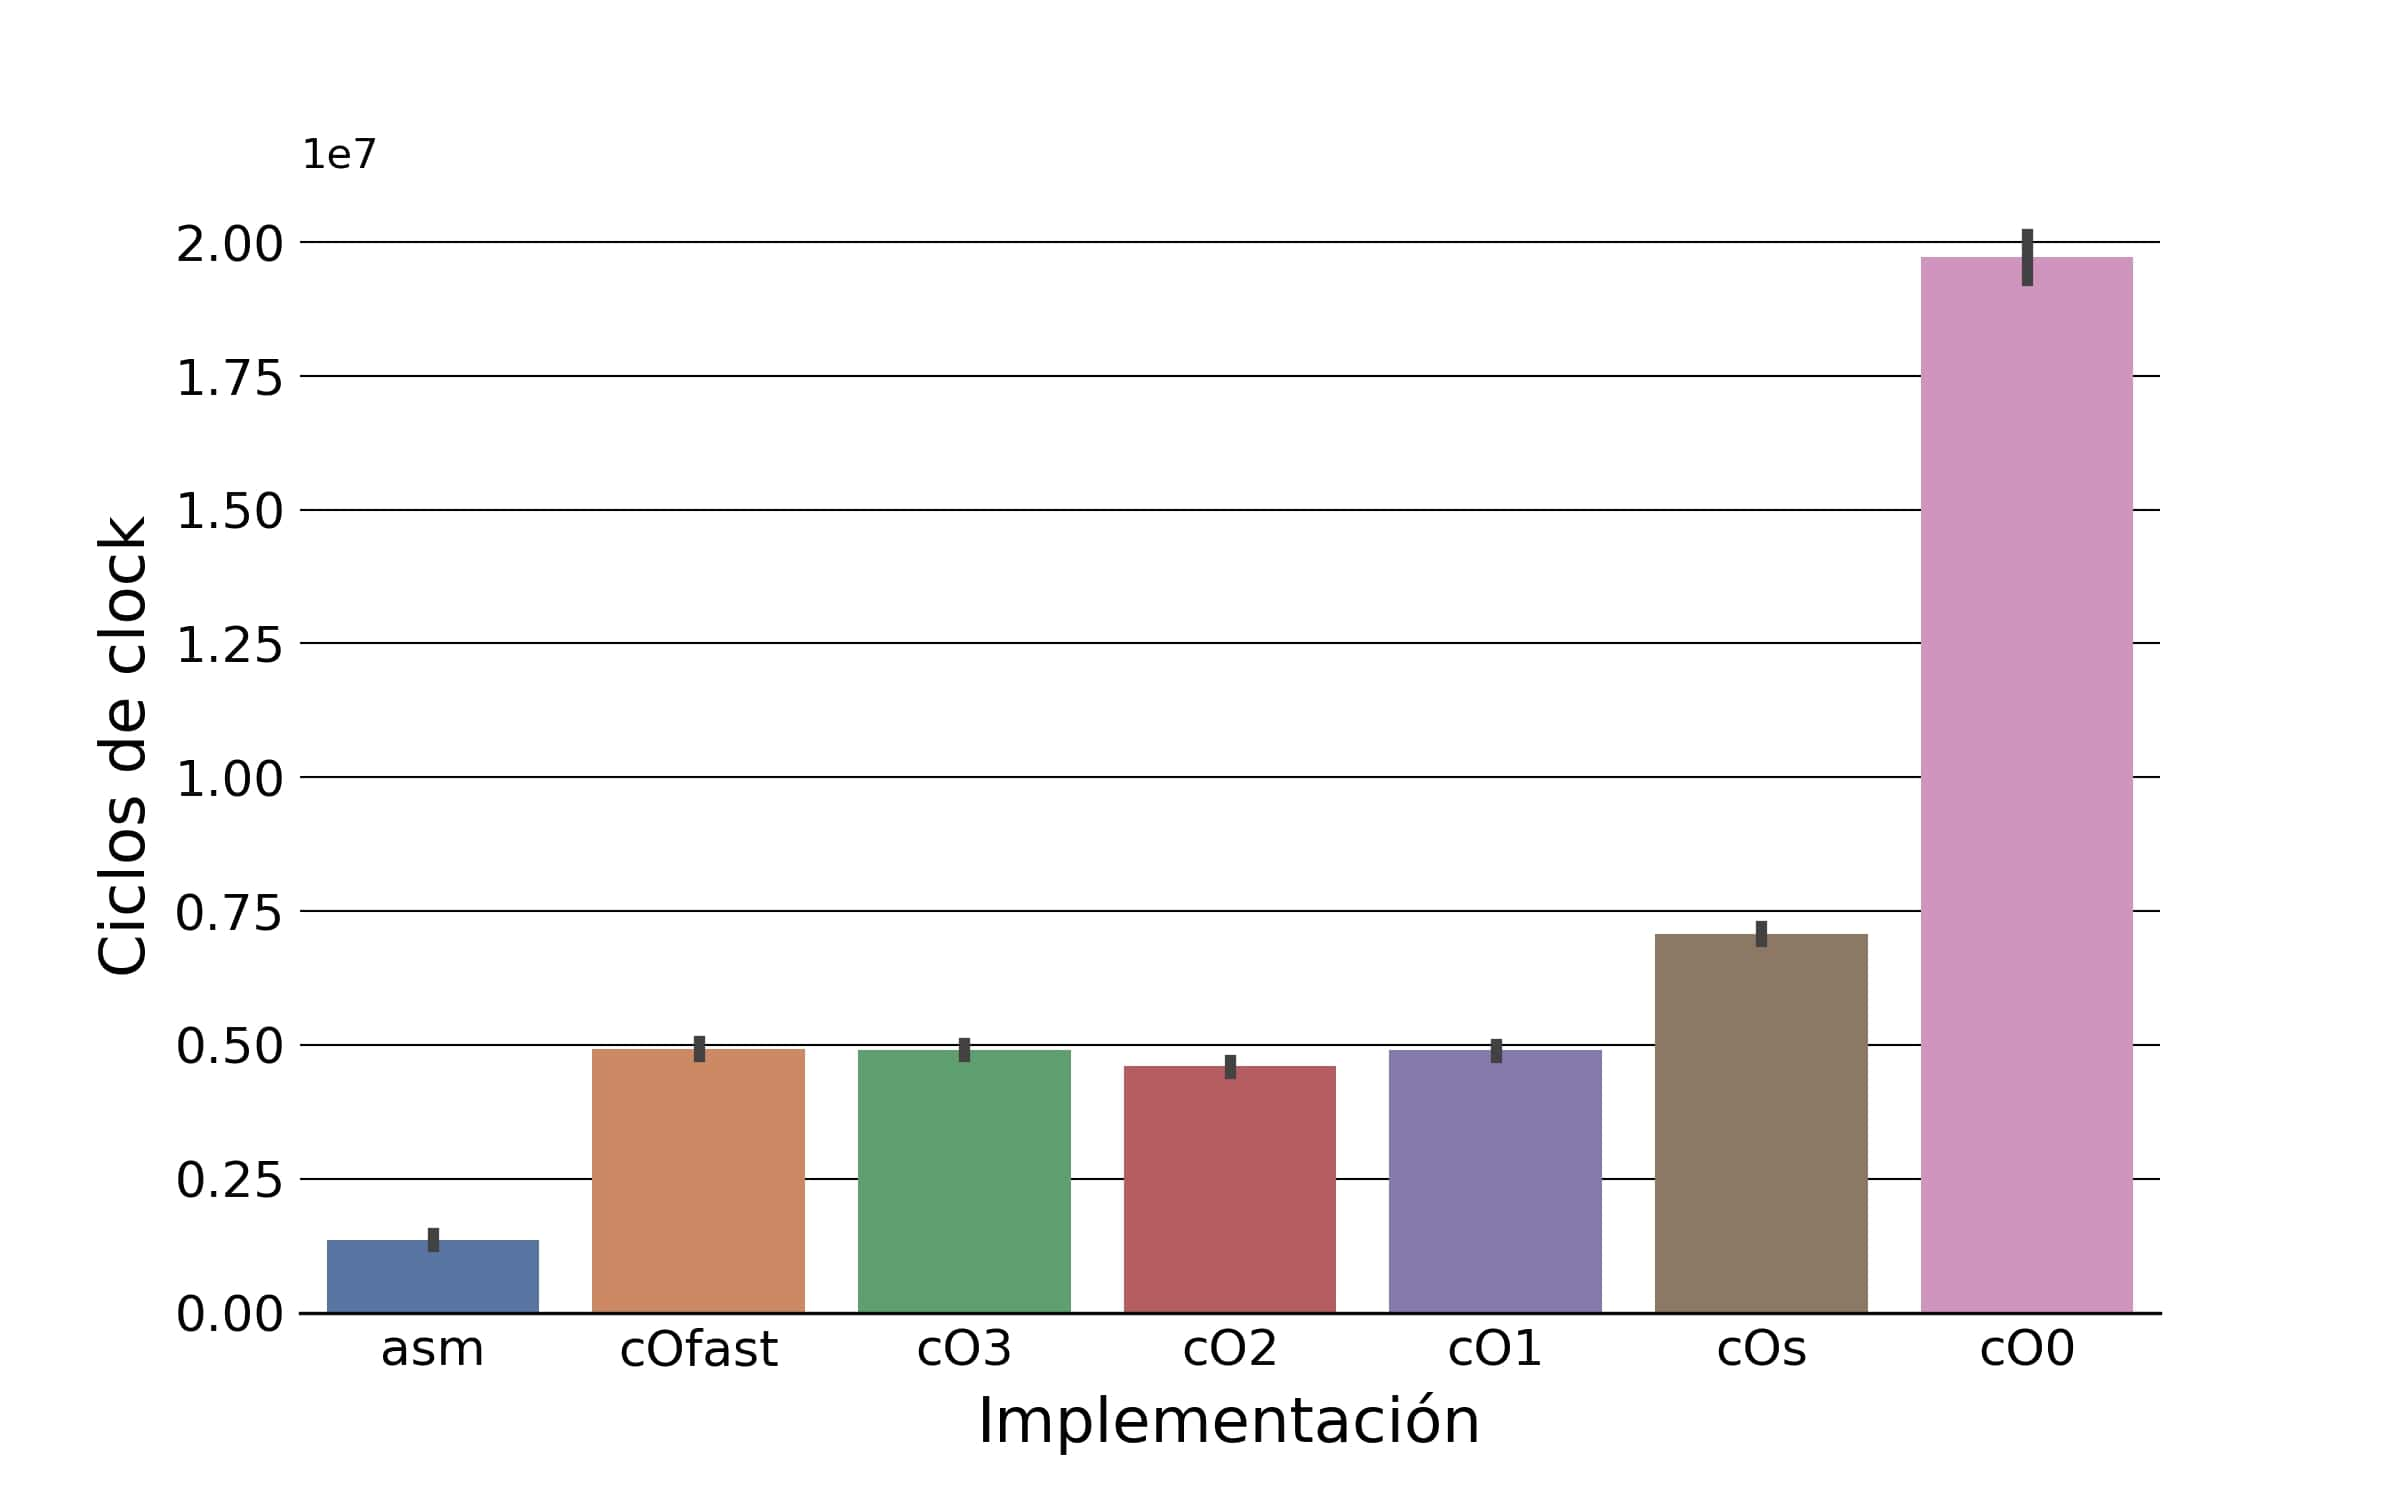
\includegraphics[scale=0.1]{img/exp0ocultar.jpg}
	\caption{Comparación C vs ASM: Ocultar}
  \end{center}
\end{figure}


Los resultados para \textit{Descubrir} son similares (figura 19): la implementación en Assembler es un 71.45\% más rápida que la mejor implementación de C, que en este caso fue cO$\textsubscript{fast}$. La media para assembler fue de 1030321 ciclos, con un desvío estándar de 91973, mientras que la media para cO$\textsubscript{fast}$ fue de 3603605, con un desvío de 88655. En este caso, los flags de compilación cO$\textsubscript{2}$, cO$\textsubscript{3}$ y cO$\textsubscript{fast}$ arrojaron prácticamente los mismos resultados.

\begin{figure}[!htb]
  \begin{center}
	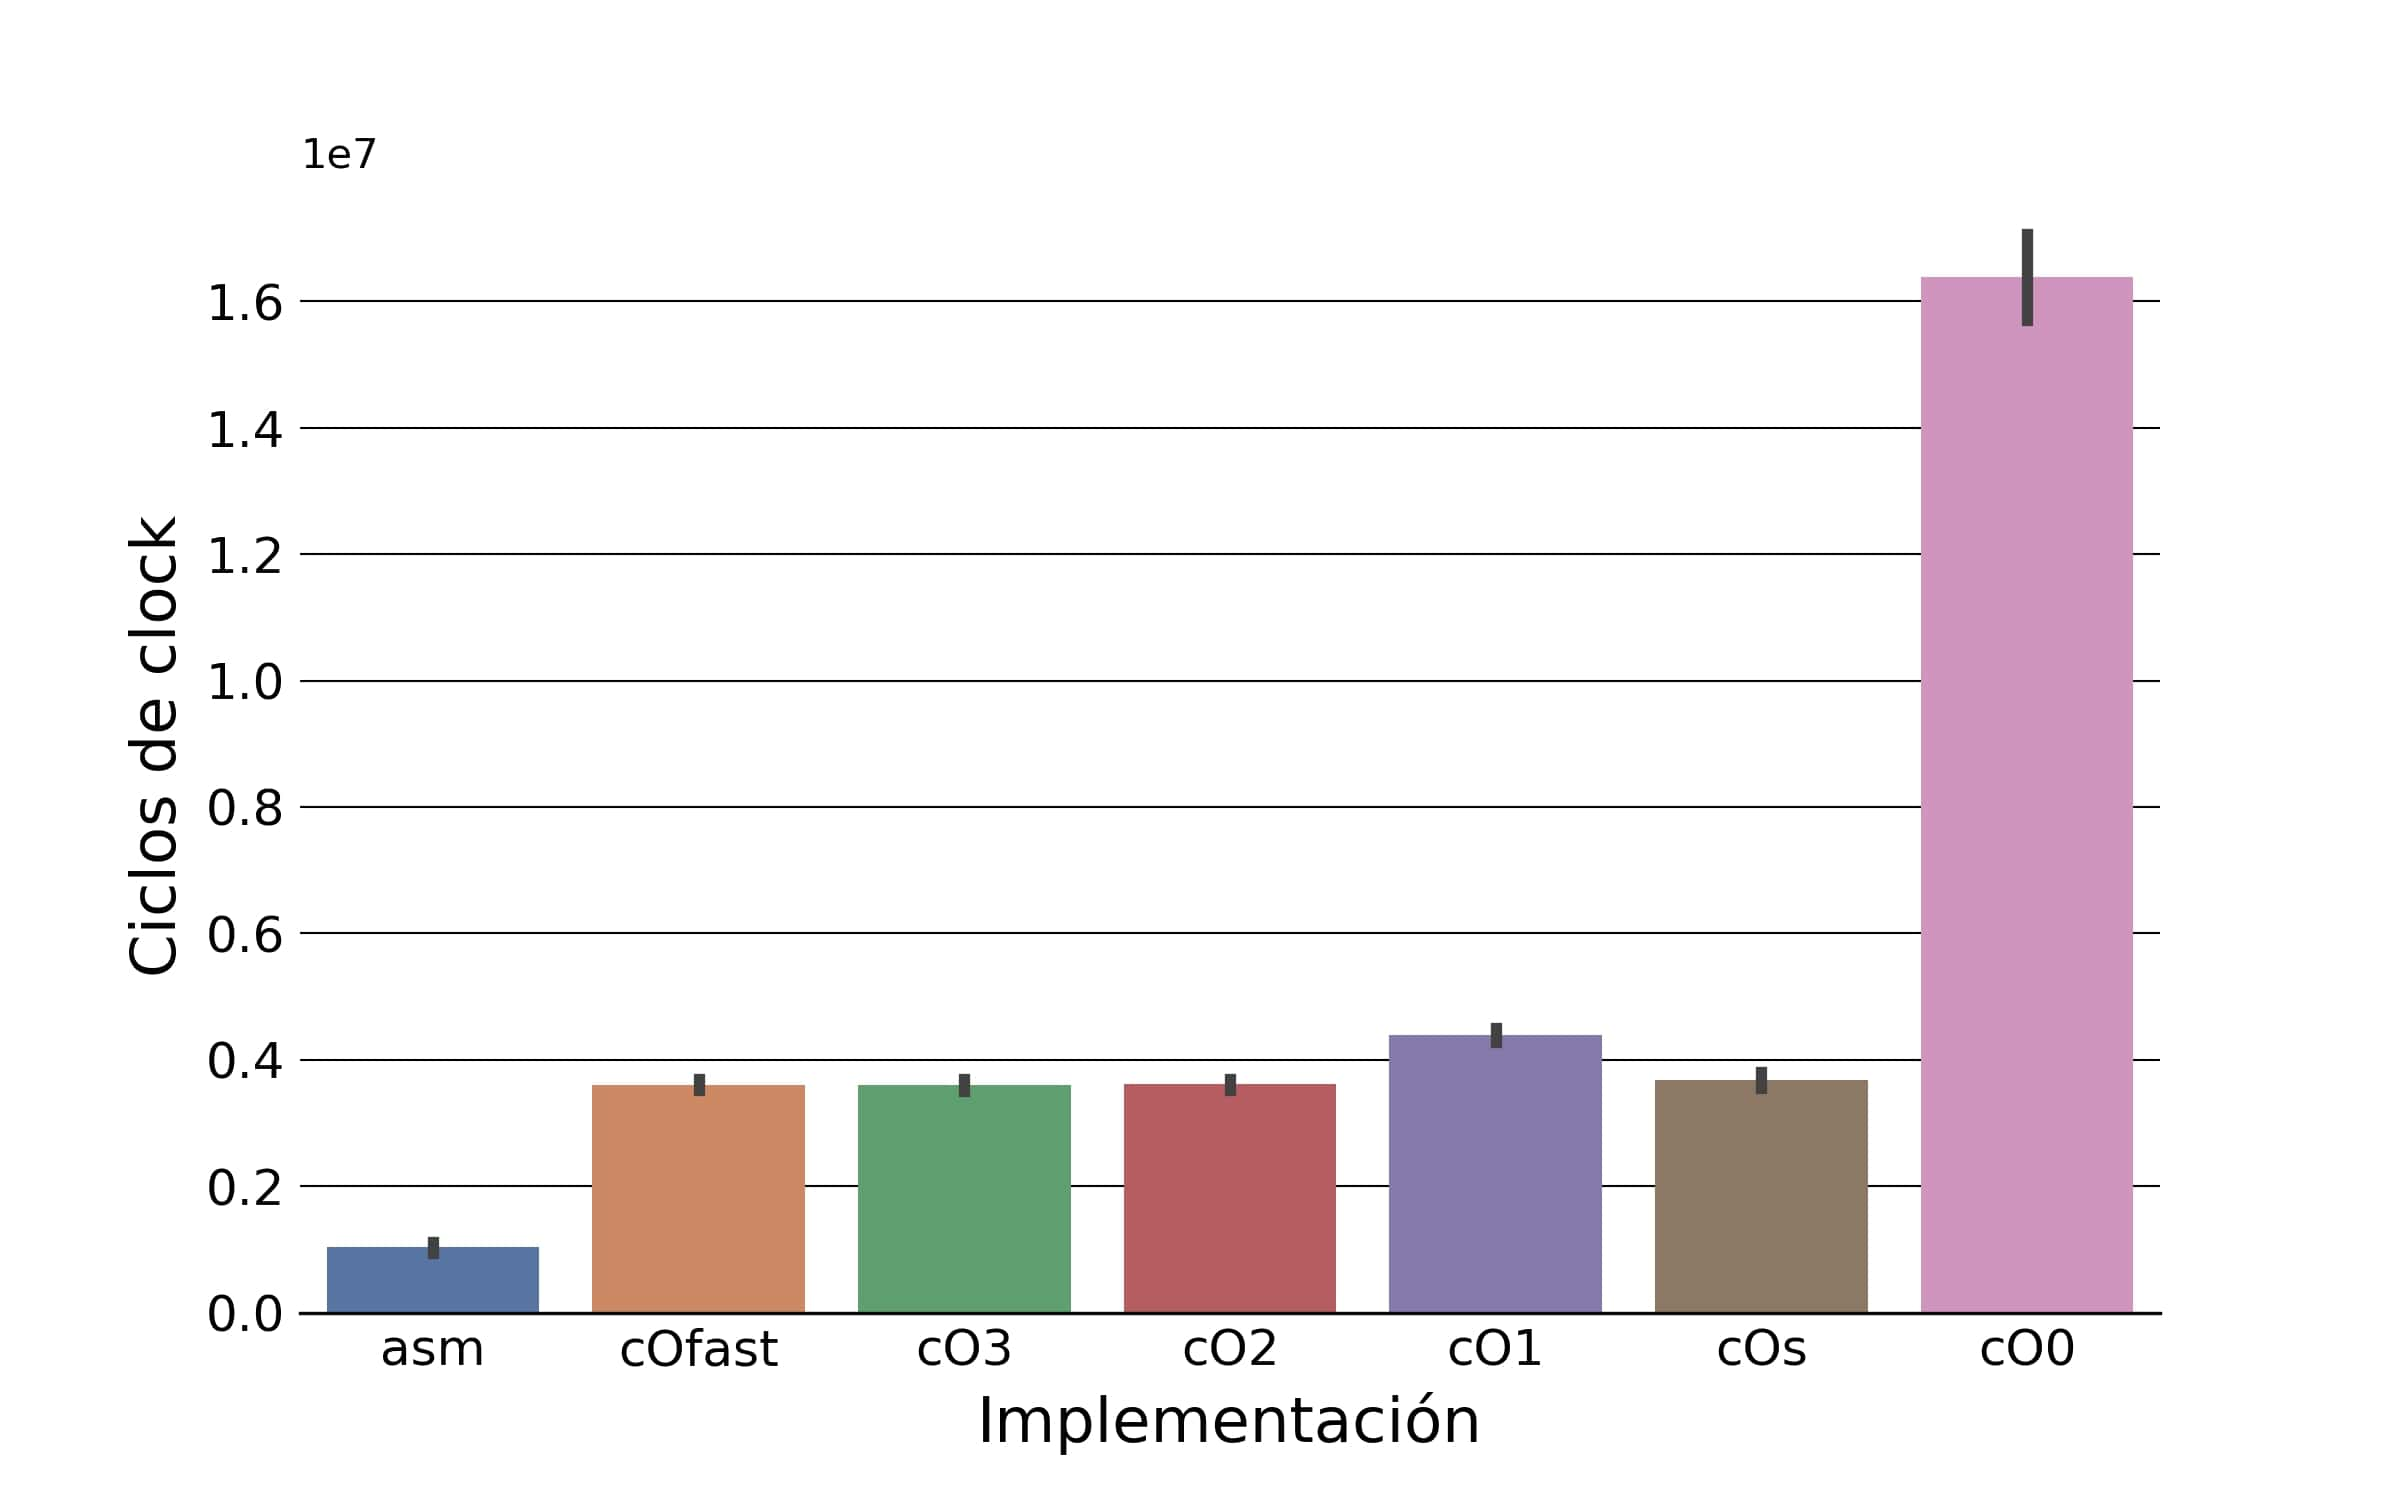
\includegraphics[scale=0.1]{img/exp0descubrir.jpg}
	\caption{Comparación C vs ASM: Descubrir}
  \end{center}
\end{figure}

Finalmente, en \textit{Zigzag} el porcentaje de optimización de assembler fue algo menor, de un 51.71\% respecto de la mejor versión de C, que en este caso también fue cO$\textsubscript{fast}$ (prácticamente al mismo nivel que cO$\textsubscript{2}$ (figura 20).

\begin{figure}[!htb]
  \begin{center}
	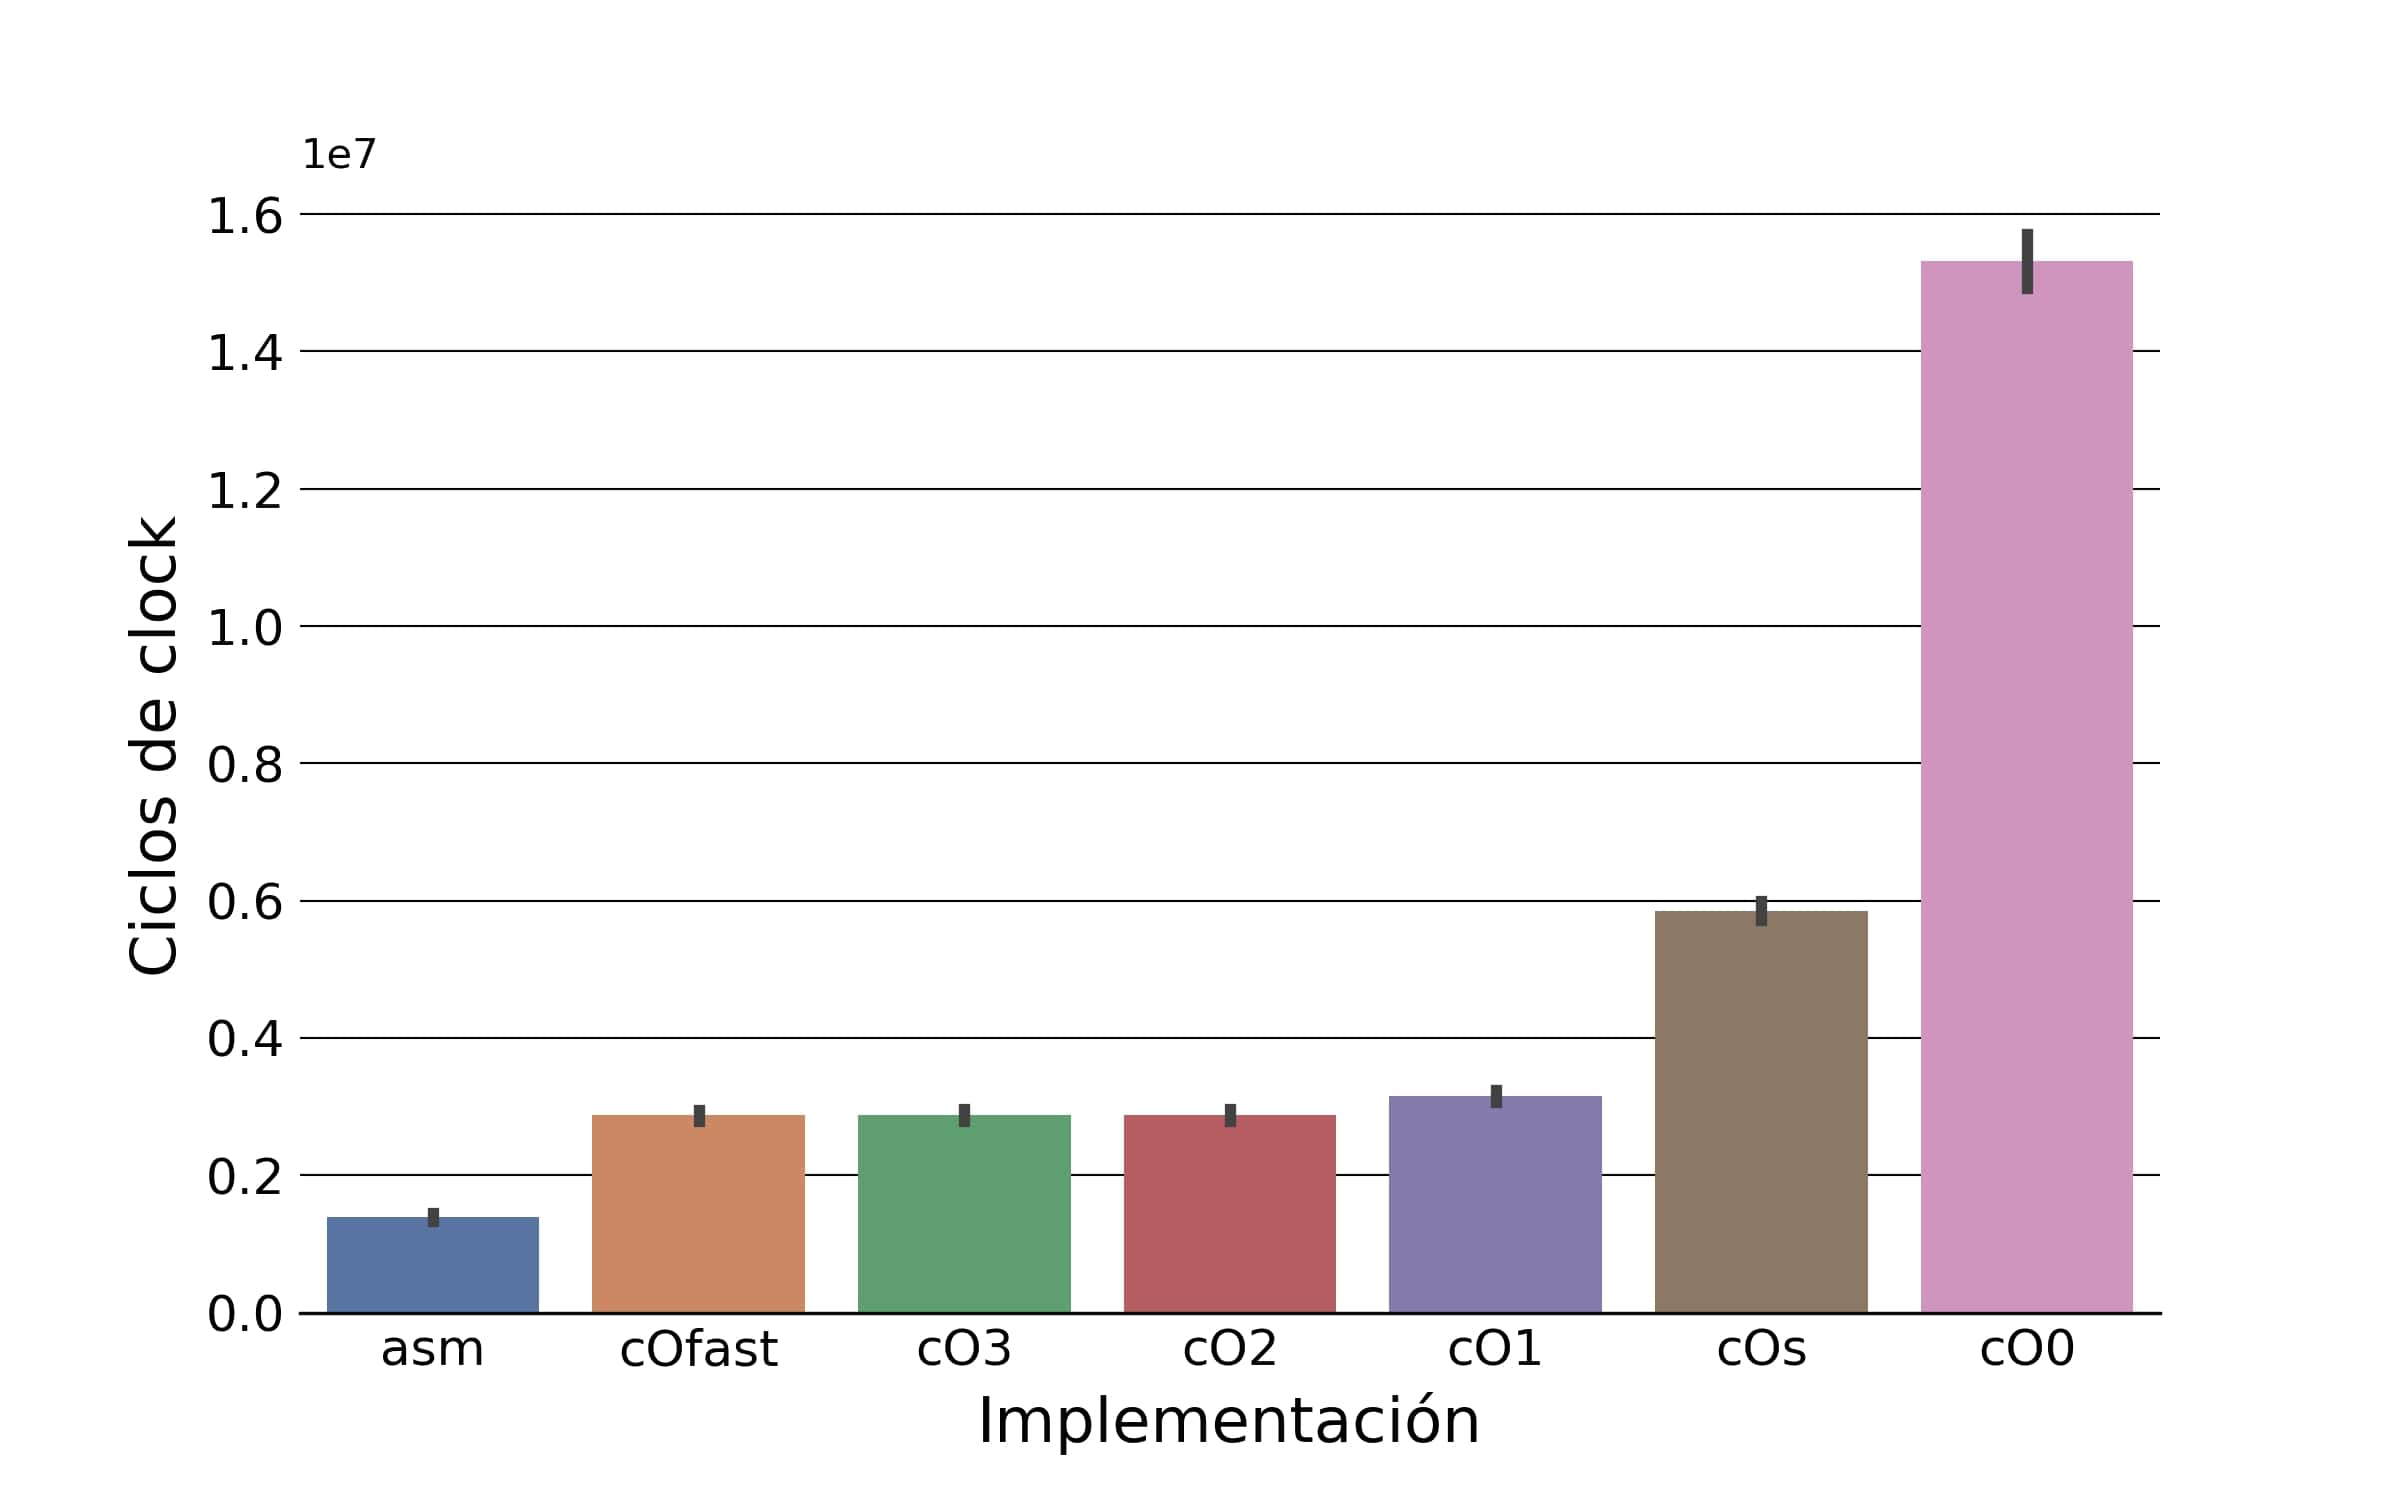
\includegraphics[scale=0.1]{img/exp0zigzag.jpg}
	\caption{Comparación C vs ASM: Zigzag}
  \end{center}
\end{figure}

Estos resultados confirman que las implementaciones en Assembler con SIMD son mucho más óptimas que cualquier implementación en las C, lo cual tiene su explicación en el procesamiento en simultáneo.

\subsection{Experimento 1: Desenrollar ciclos}
\subsubsection{Descripción del problema}
Una de las técnicas utilizadas habitualmente para mejorar la performance es la de desenrollar ciclos o \textit{loop unrolling}. Consiste en extender los ciclos para eliminar saltos e instrucciones de control (eliminando así las \textit{branch penalties}) y en general permite mejorar la performance temporal a costa de aumentar el tamaño del código. \\
Si bien en los tres filtros el costo del ciclo en relación con los accesos a memoria y el procesamiento es pequeño, es posible que pueda observarse una leve optimización. \\
El objetivo de este experimento es hallar el punto óptimo de \textit{unrolling} para cada filtro.
Los experimentos se realizaron sobre una imagen de 1600x800 para poder desenrollar hasta 16 ciclos sin necesidad de incluir instrucciones de control de ciclo en el medio (es decir, para asegurar que los píxeles de la imagen son múltiplo de la cantidad de píxeles procesados en un ciclo desenrollado). En las filas pares de \textit{Zigzag}, sin embargo, se mantuvo la comparación de control de ciclo entre los \textit{unrollings} ya que para evitarla era necesario agregar casos bordes extensos que tendrían un efecto mucho maś significativo en la performance que la comparación. \\
En \textit{Zigzag}, además, el primer \textit{unrolling} consistió en repetir el código correspondiente a las filas pares y evitar los saltos del distribuidor de filas. Luego, como tiene tanto ciclos internos como externos, se realizaron dos tipos de \textit{unrollings}: por ciclos internos y ciclos externos.

\subsubsection{Hipótesis}
Dado que los filtros tienen características diferentes, es probable que el punto óptimo sea diferente. En particular, dado que \textit{Ocultar} y \textit{Descubrir} son prácticamente iguales en cuanto al funcionamiento del ciclo, es esperable que se comporten de manera diferente a \textit{Zigzag}, que tiene muchos más saltos en los que se evalúan varias condiciones, además de ciclos internos. \\
En el caso de \textit{Zigzag}, se espera que el efecto sea más pronunciado ya desde los primeros \textit{unrollings}, dado que es el filtro en el que el ciclo es el que tiene el costo relativo más alto. 
\subsubsection{Resultados}
En el caso de \textit{Ocultar}, el valor en ciclos más bajo se registró al desenrollar los ciclos en 4; sin embargo, la diferencia es insignificante en relación con la versión original: el porcentaje de optimización es de 0.12\%. Como se puede ver en la figura 21, la versión original y las desenrolladas 2, 4 y 8 veces tuvieron un rendimiento prácticamente idéntico, que bajó significativamente al desenrollar por 16.

\begin{figure}[!htb]
  \begin{center}
	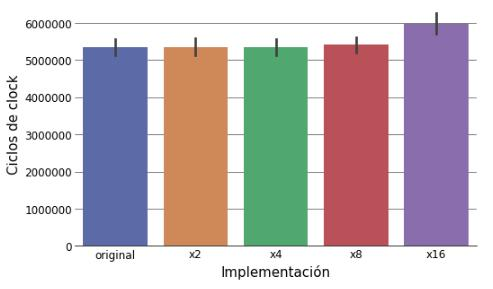
\includegraphics[scale=0.7]{img/exp1ocultar.jpg}
	\caption{Desenrollar ciclos: Ocultar}
  \end{center}
\end{figure}

\textit{Descubrir} arrojó resultados muy similares, aunque en este caso el porcentaje de optimización de la mejor versión respecto de la original fue superior: 2.56\%. Aquí también se puede ver que entre las primeras 4 implementaciones prácticamente no hay diferencias, mientras que la última tiene un rendimiento significativamente más bajo (figura 22).

\begin{figure}[!htb]
  \begin{center}
	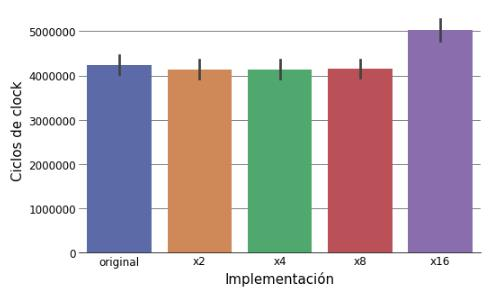
\includegraphics[scale=0.7]{img/exp1descubrir.jpg}
	\caption{Desenrollar ciclos: Descubrir}
  \end{center}
\end{figure}

En \textit{Zigzag} el mejor rendimiento se obtuvo al desenrollar los ciclos internos en 2. Todas las versiones desenrolladas son ligeramente más óptimas que la original, pero la diferencia es mínima. El porcentaje de optimización de la mejor versión es de 1.40\% (figura 23).

\begin{figure}[!htb]
  \begin{center}
	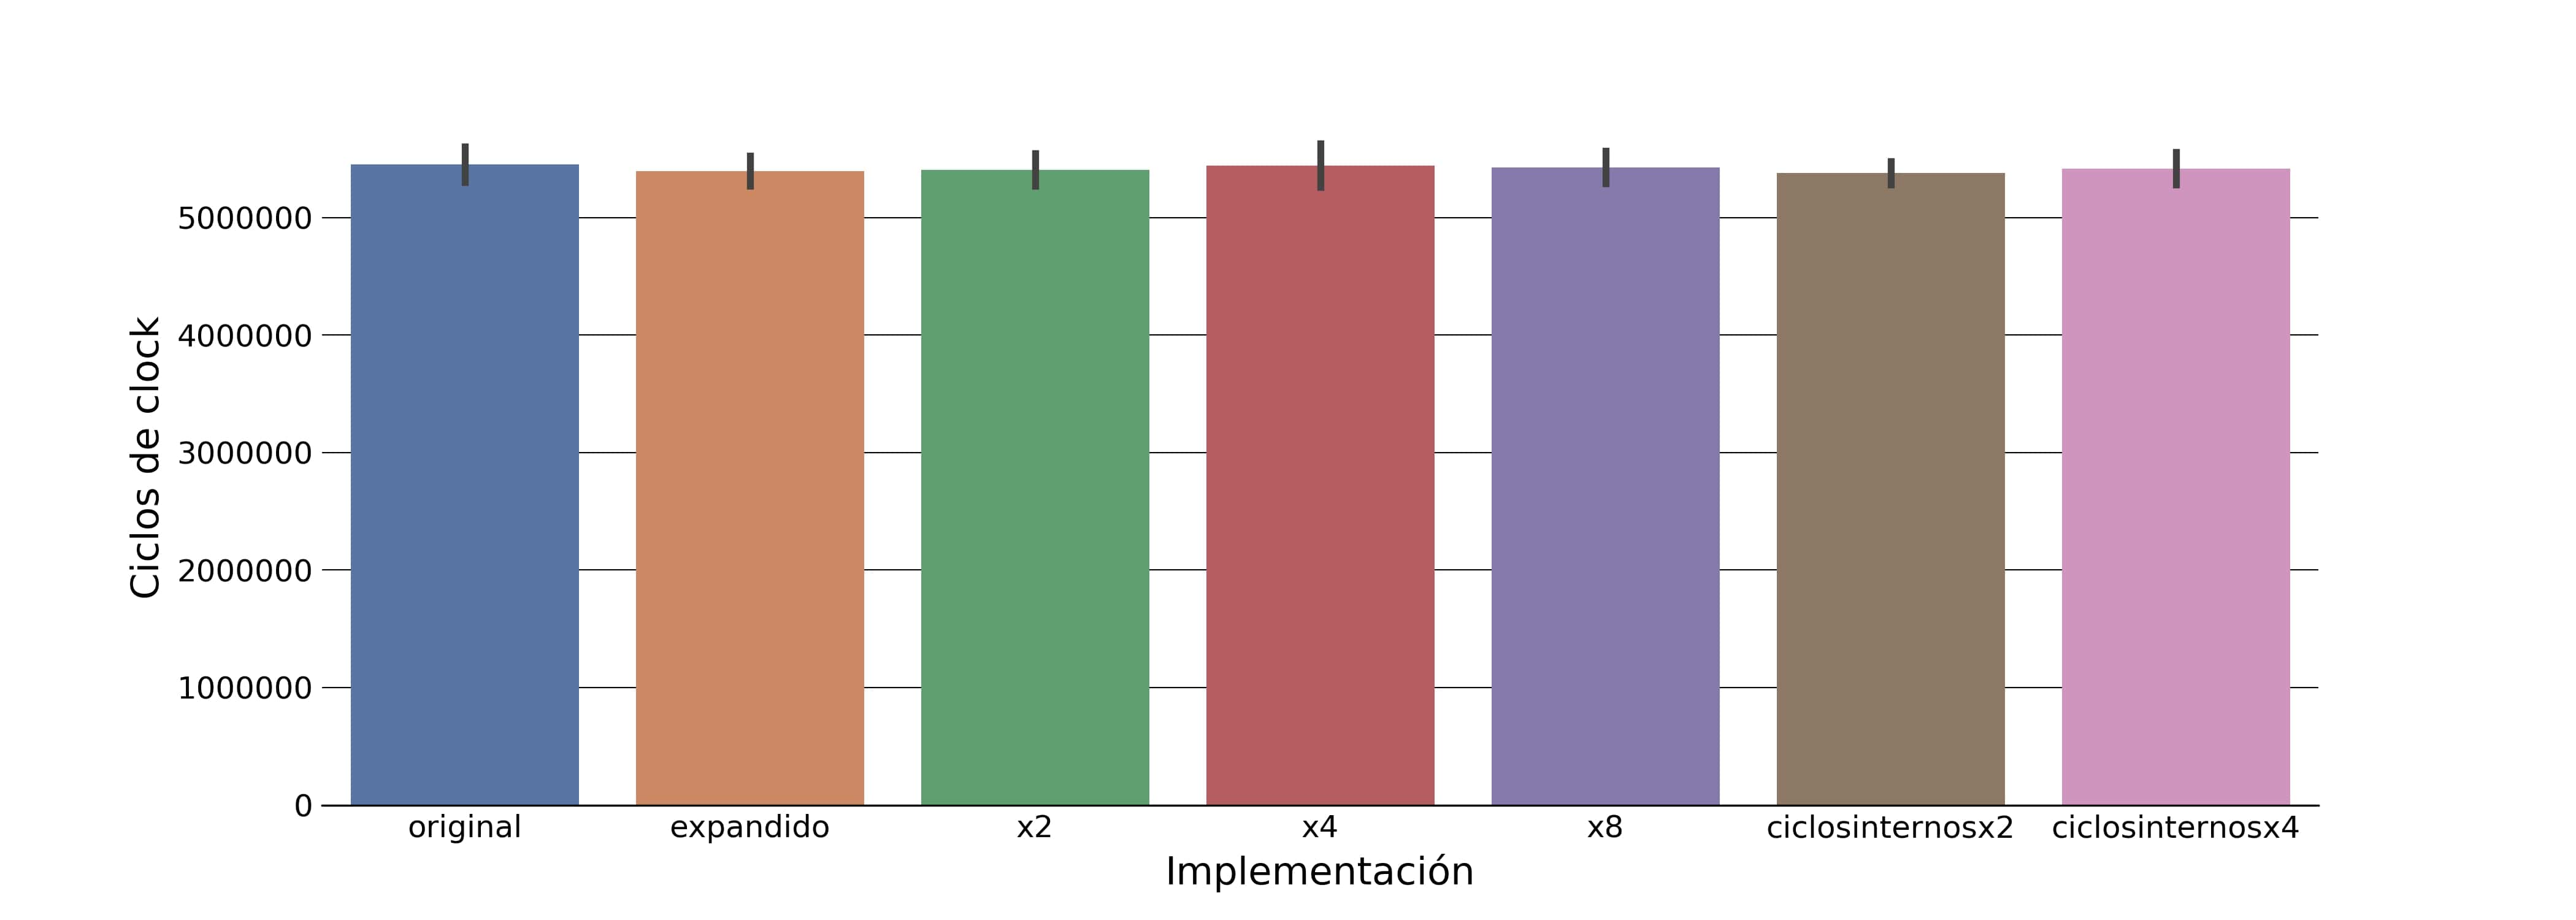
\includegraphics[scale=0.1]{img/exp1zigzag.jpg}
	\caption{Desenrollar ciclos: Zigzag}
  \end{center}
\end{figure}

Aunque se esperaba que la optimización fuera leve, a diferencia de lo que se planteó en la hipótesis los resultados obtenidos muestran que desenrollar ciclos no es una buena estrategia para mejorar la performance, ni siquiera en el caso de \textit{Zigzag}. Además de lo ya mencionado, esto también podría deberse a otros factores. En primer lugar, es probable que esté relacionado con las características del procesador, ya que los procesadores más modernos están diseñados para manejar de manera más óptima los saltos y \textit{branches}. Otra causa posible es que este tipo de optimización tenga efecto en ciclos cortos, con pocas líneas de código, ya que en funciones más largas es probable que el tradeoff tiempo-espacio empiece a jugar un rol importante ya al desenrollar por 2. Esto explicaría que en \textit{Descubrir} se haya obtenido una optimización muy reducida pero mayor que en los otros casos.

\subsection{Experimento 2: Extender ciclos}
\subsubsection{Descripción del problema}
A partir de los resultados del experimento anterior, se consideró otra opción para optimizar los ciclos de \textit{Ocultar} y \textit{Descubrir}: trabajar con 16 píxeles por ciclo en lugar de 8. Esta opción además de reducir los ciclos a la mitad podría representar una optimización adicional ya que permite reducir la cantidad de instrucciones totales. Esto ocurre porque algunas de las instrucciones (como el shift de maścaras) se realizan una sola vez en cada ciclo independientemente de la cantidad de registros {\tt xmm} a las que se apliquen. \\
En \textit{Ocultar}, además, tiene la ventaja adicional de que el registro {\tt xmm} donde se almacenaban los píxeles ya convertidos a escala de grises tenía espacio para 8 píxeles más, que no estaba siendo aprovechado al trabajar con 8 píxeles por ciclo. \\
La desventaja de esta opción es que en este caso es necesario asumir que el ancho de las imágenes es múltiplo de 16 píxeles, podría ser una buena opción para los casos en los que esta condición se cumple. Además, esta restricción adicional también aplicaba al caso de desenrollar ciclos.

\subsubsection{Hipótesis}
Trabajar con 16 píxeles por ciclo en lugar de 8 mejora la performance de ambos filtros y representa una mejor optimización que desenrollar ciclos.

\subsubsection{Resultados}
Para \textit{Ocultar} se obtuvo una media de 1364914 con un desvío estándar de 102661 para la implementación que procesa 8 píxeles y una media de 1344083 con un desvío de 106279 para la de 16 (figura 24). El porcentaje de optimización fue mucho menor a lo esperado, de 1.53\%, pero aun así fue más alto que el obtenido al desenrollar. En cambio, en \textit{Descubrir} la optimización fue mayor: 5.34\%. Para 8 píxeles la media fue de 1013008 con un desvío 83064 mientras que para 16 la media fue de 958974 con un desvío de 93991 (figura 25).

\begin{figure}[!htb]
   \begin{minipage}{0.48\textwidth}
     \centering
     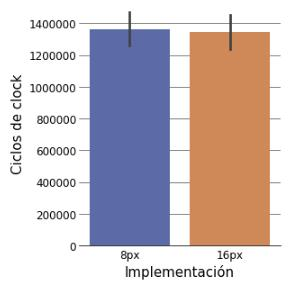
\includegraphics[width=.7\linewidth]{img/exp2ocultar.jpg}
     \caption{8 vs 16 píxeles: Ocultar}
   \end{minipage}\hfill
   \begin{minipage}{0.48\textwidth}
     \centering
     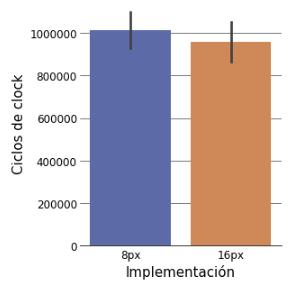
\includegraphics[width=.7\linewidth]{img/exp2descubrir.jpg}
     \caption{8 vs 16 píxeles: Descubrir}
   \end{minipage}
\end{figure}

En síntesis, si bien el nivel de optimización no fue el esperado, esta estrategia tuvo un efecto más significativo que desenrollar, además de tener otras ventajas, como aumentar en menor medida el tamaño del código y no afectar la legibilidad. Otro punto a destacar es que la optimización fue mayor en \textit{Descubrir}. Allí, el procesamiento tiene un costo relativo mayor que en \textit{Ocultar}, y algunas de las instrucciones de la reorganización de bits con máscaras, que conforman la mayor parte del procesamiento, se realizan una única vez por ciclo independientemente de la cantidad de píxeles procesados.

\subsection{Experimento 3: Optimizar accesos a memoria}
\subsubsection{Descripción del problema}

Otro aspecto que es importante tener en cuenta en cualquier intento de optimización son los accesos a memoria, ya que son operaciones muy costosas en términos temporales. \\
Las implementaciones originales de los filtros ya están lo más optimizadas posible en términos de la cantidad de accesos, ya que en ningún momento se realizan accesos innecesarios o se levanta información repetida. Por este motivo, lo que resta analizar es el modo de acceso. \\
Si la posición de memoria a la que se quiere acceder está alineada a 16 bytes, es posible realizar accesos más rápidos mediante la instrucción {\tt movdqa}. En algunos casos esto ya está dado, pero en otros puede ser costoso garantizar esa alineación. Por eso, puede ser útil analizar la mejora en la performance que la utlización de esta instrucción produce en comparación con {\tt movdqu}. \\
Los accesos a memoria también son costosos por los pasos que involucra guardar los datos en la memoria caché. Por este motivo vale la pena considerar dos instrucciones que permiten evitar este proceso: {\tt movntdqa} y {\tt movntdq}. \\
{\tt movntdqa} carga 128 bits desde memoria a un registro {\tt xmm} usando la técnica de {\tt write combining}\footnote{Ver Intel (November 1998) "Write Combining Memory Implementation Guidelines". \\ http://download.intel.com/design/PentiumII/applnots/24442201.pdf}, que permite que los datos sean almacenados temporalmente en un buffer y que luego se escriban todos juntos, en lugar de escribirse individualmente o en partes. {\tt movntdq} utiliza la misma técnica para escribir en memoria. Ambas permiten reducir el uso de la caché, lo que podría resultar en una mejora del rendimiento. Sin embargo, puede causar problemas, especialmente al realizar operaciones de lectura.\footnote{Ver https://fgiesen.wordpress.com/2013/01/29/write-combining-is-not-your-friend} Por lo tanto, evaluaremos también una implementación que utilice estas dos instrucciones y otra que solo utilice \textit{write combining} para escribir a memoria. \\
En este experimento evaluamos implementaciones de los filtros \textit{Ocultar} y \textit{Descubrir} donde se utilizan estas alternativas de acceso a memoria. Dado que en estos filtros los accesos ya se encuentran alineados, para evaluar la condición {\tt movdqu} se realizó un desplazamiento de dos píxeles y, para no agregar casos borde que pudieran afectar los resultados, se decidió finalizar el ciclo una iteración antes de llegar al fin de la imagen. Es decir que quedan 8 píxeles sin procesar, condición que se replicó en todas las otras variantes para que los tiempos de procesamiento de todas las condiciones fueran equiparables. No incluimos \textit{Zigzag} ya que el algoritmo de base para la implementación este filtro requiere recorrer las imágenes con desfasajes y esto hace que los accesos estén desalineados necesariamente.

\subsubsection{Hipótesis}
Las implementaciones que acceden a memoria de forma alineada serán más óptimas que las que acceden de forma no alineada, pero es probable que el efecto no sea tan significativo como para justificar el costo de realizar operaciones adicionales para garantizar la alineación (como requeriría el caso de \textit{Zigzag}). Los accesos con \textit{write combining} sí serán significativamente más eficientes ya que reducirán el costo asociado a las operaciones de caché.

\subsubsection{Resultados}
En \textit{Ocultar} los resultados estuvieron en línea con lo esperado. Las implementaciones con {\tt movdqa} y {\tt movdqu} prácticamente no registraron diferencias, mientras que las implementaciones con {\tt movntdq} y {\tt movntdqa} resultaron significativamente más óptimas: un 13.57\% respecto de la implementación con {\tt movdqa}, es decir, la versión original (figura 26).

\begin{figure}[!htb]
  \begin{center}
	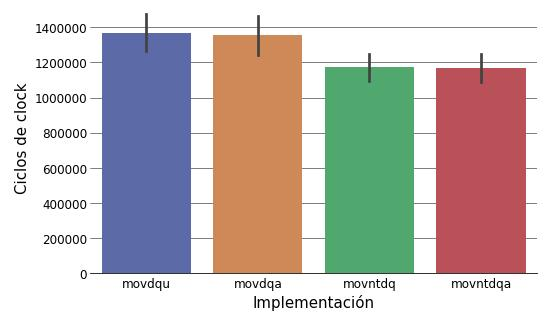
\includegraphics[scale=0.6]{img/exp3ocultar.jpg}
	\caption{Optimización de accesos a memoria: Ocultar}
  \end{center}
\end{figure}

En cambio, en \textit{Descubrir} no se observó este efecto. De hecho, aunque la implementación con {\tt movdqa} mostró una ventaja muy leve respecto de las otras, las cuatro implementaciones tuvieron prácticamente el mismo rendimiento, como se puede observar en la figura 27.

\begin{figure}[!htb]
  \begin{center}
	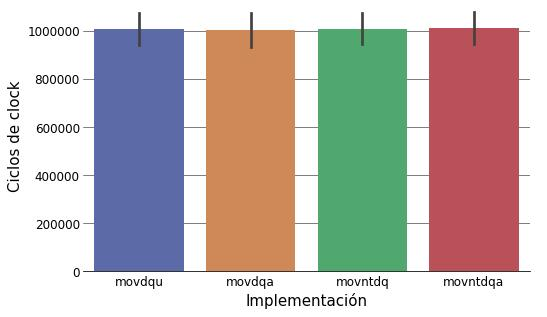
\includegraphics[scale=0.6]{img/exp3descubrir.jpg}
	\caption{Optimización de accesos a memoria: Descubrir}
  \end{center}
\end{figure}

A diferencia de lo que se planteó en la hipótesis, casi no parece haber diferencias entre los accesos alineados y no alineados. Es posible que esto se deba a que los accesos a memoria en estos filtros son relativamente reducidos. Sin embargo, las diferencias en \textit{Ocultar} con las instrucciones que utilizan \textit{write combining} son importantes, pero no así en \textit{Descubrir}. Esto podría tener su explicación en el hecho de que en el primero se está levantando información de dos fuentes distintas, por lo que evitar operaciones de caché en este caso tendría un efecto mayor, mientras que en el segundo esto no ocurre. Además, como se observó al analizar el costo relativo de los accesos a memoria, en \textit{Ocultar} representan casi un 92\% mientras que en \textit{Descubrir} solo un 66\%, por lo cual es esperable que este tipo de optimizaciones tengan efecto en el primero.

\subsection{Experimento 4: Reemplazar división en float por división entera}
\subsubsection{Descripción del problema}
En el análisis del costo relativo de los accesos a memoria, el ciclo y el procesamiento de los píxeles, \textit{Zigzag} se destacó por ser el filtro en el que el procesamiento requería más ciclos de clock en relación a los requeridos por las otras operaciones. Por este motivo, optimizar el procesamiento en este caso podría tener un efecto significativo sobre el rendimiento del filtro. \\
Al realizar la división para calcular el promedio en las filas pares de \textit{Zigzag}, en la implementación original se realiza una conversión a float ya que no existe una instrucción SIMD para la división entera. Además, como los enteros a dividir son de 16 bits y los floats de precisión simple son de 32, para poder realizar esta conversión es necesario hacer también operaciones de empaquetado y desempaquetado, y aplicar la división sobre 4 registros en lugar de 2. \\
Sin embargo, existe una técnica que permite dividir enteros utilizando la multiplicación. Si quiere calcular $\frac{x}{d}$ y $d$ es una constante ya conocida, tomando un número real positivo m se puede reescribir $\frac{x}{d}$ como
\begin{equation}
\frac{x\cdot\frac{m}{d}}{m}
\end{equation}
Si $m$ fuese divisible por $d$, y $m$ una potencia de dos, la división $\frac{m}{d}$ se podría hacer con un shift. Sin embargo, incluso si este no es el caso, se puede hacer una manipulación algebraica para que esto sea posible, 1) hallando un $n$ tal que $\frac{m+n}{d}$ sea un entero, donde $n < d$ y $m + n \equiv 0 \Mod{d}$ y 2) buscando un $m$ que sea potencia de dos. \\
Para cumplir con la condición 1, se reemplaza $m$ por $m+n$ y luego, distribuyendo x, se obtiene lo siguiente: 
\begin{equation}
\frac{x\cdot\frac{m+n}{d}}{m} = \frac{x\cdot\frac{m}{d}}{m} + \frac{x\cdot\frac{n}{d}}{m}
\end{equation}

Como se indicó antes, el primero de estos dos términos es igual a $\frac{x}{d}$. En cuanto al segundo término, si se logra que este sea menor a $\frac{1}{d}$, independientemente del valor de $x$, la parte entera de $\frac{x}{d}$ + $\frac{x\cdot\frac{n}{d}}{m}$ será igual que la parte entera de $\frac{x}{d}$. Así, se agrega una tercera condición: hallar un $m$ lo suficientemente grande para que el segundo término sea menor a $\frac{1}{d}$. \\
En síntesis, sea  $\frac{m+n}{d} = z$. Entonces,
\begin{equation}
x\cdot z = x\cdot\frac{m}{d} + x\cdot\frac{n}{d}
\end{equation}
y
\begin{equation}
\frac{x\cdot z}{m} = \frac{x}{d} + \frac{x\cdot\frac{n}{d}}{m}
\end{equation}
donde $\frac{x}{d}$, el primer término, es la parte entera y el segundo la parte decimal, que se descarta.

En \textit{Zigzag}, se divide la suma de 5 bytes por 5. Por lo tanto, el máximo valor posible de $x$ es $255\cdot 5$. A su vez, $n \leq 4$ (ya que es el máximo valor posible módulo 5). Es decir, hay que hallar un $m$ tal que $\frac{255\cdot4}{m}$ sea menor a $\frac{1}{5}$. El primer número que cumple esta condición es $2^{13}$. Sin embargo, para evitar unir las partes baja y alta de la multiplicación, se optó por tomar $m = 2^{16} = 65536$ y $z = \frac{65536 + 4}{5} = 13108$, y así poder descartar la parte baja en su totalidad. \\

Para comparar el costo de la conversión a float y la división con {\tt divps} frente a la división entera con {\tt mulhw} y poder considerarlo independientemente del costo de las operaciones de desempaquetado y empaquetado, se evaluaron dos implementaciones alternativas del filtro: una con la división entera con instrucciones de empaquetado de relleno (es decir, solo se eliminan las conversiones a float y se reemplaza {\tt divps}), y otra con la división entera sin ninguna instrucción innecesaria, que representa el resultado real de la optimización.

\subsubsection{Hipótesis}
Dado que las conversiones a float son costosas, utilizar la división entera y evitar las conversiones será más óptimo que hacer la división en float, incluso manteniendo las operaciones de (des)empaquetado. La implementación con la división entera sin instrucciones adicionales será, lógicamente, la más óptima, ya que reduce la cantidad de instrucciones por ciclo.

\subsubsection{Resultados}
Como se puede ver en la figura 28, la implementación con división entera sin (des)empaquetados fue la que obtuvo el mejor rendimiento, con un 18.15\% de optimización respecto de la original. La versión con las instrucciones de relleno fue más óptima que la original pero la diferencia fue muy pequeña: solo un 1.35\% de optimización, lo cual indica que la ventaja fundamental de utilizar la división entera en este caso no es una reducción importante en el costo de las instrucciones en sí mismas sino el procesamiento adicional que se puede evitar al utilizarla.

\begin{figure}[!htb]
  \begin{center}
	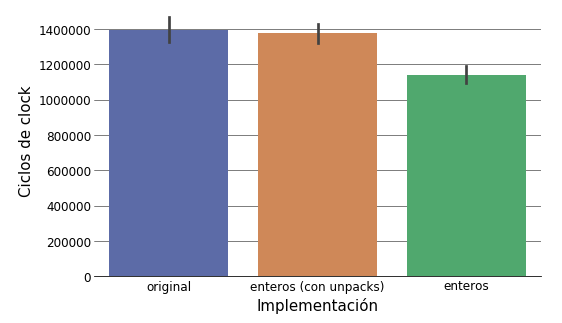
\includegraphics[scale=0.6]{img/exp4diventera.png}
	\caption{Zigzag: Comparación división float con división entera}
  \end{center}
\end{figure}

A su vez, que se haya obtenido un porcentaje significativo de optimización al tratar de reducir el costo de procesamiento se corresponde con lo observado al realizar el análisis del costo relativo de cada parte de los filtros, ya que en \textit{Zigzag} era el procesamiento de los píxeles lo que ocupaba la mayor parte de los ciclos de clock.

\newpage
\section{Conclusión}

Del proceso de implementación de los filtros y de experimentación sobre sus variantes, es posible concluir que el modelo de procesamiento SIMD posee una clara ventaja frente al modelo SISD en cuanto a su rendimiento temporal. Como se observó, en todos los casos las implementaciones en Assembler son significativamente más rápidas que las de C, reduciendo los tiempos de procesamiento a menos de la mitad, incluso en comparación con las opciones más rápidas del compilador. Sin embargo, es posible que utilizar este modelo no siempre sea viable; es importante tener en cuenta que programar en Assembler es mucho más costoso en términos de tiempo que en C y la legibilidad del código es menor, por lo que puede haber casos en los que estas mejoras de rendimiento no justifiquen el esfuerzo adicional que requiere el uso de este modelo. También es posible que en muchos casos la naturaleza de los datos o las características del problema dificulten el procesamiento en paralelo o hagan que los beneficios de utilizarlo no sean sustanciales. No obstante, conocer las posibilidades que provee la arquitectura SSE puede ser un recurso fundamental para resolver problemas en los que la dimensión temporal sea de suma importancia. \\
Otra conclusión importante del proceso de experimentación es que la optimización no es un proceso sencillo y directo: no hay métodos infalibles para reducir los tiempos de procesamiento (al menos no frente a implementaciones que no hagan uso innecesario de recursos de forma evidente). Las optimizaciones no siempre producen el efecto esperado. Hay múltiples factores que afectan el rendimiento, como las características del procesador o ciertas características de las entradas. Por este motivo, realizar mediciones de rendimiento en un entorno lo más controlado posible es una herramienta fundamental para evaluar las decisiones tomadas y compararlas con sus posibles alternativas. \\
Además, como se observó a partir de los resultados obtenidos, la efectividad de las optimizaciones depende de las características de cada algoritmo. Las optimizaciones más efectivas fueron diferentes para cada filtro, y estas diferencias resultaron consistentes en gran medida con el análisis preliminar del costo relativo que representaba cada aspecto. De todas las modificaciones realizadas, las que produjeron un mayor aumento del rendimiento fueron procesar de a 16 píxeles por ciclo en lugar de 8 en el caso de \textit{Descubrir}, reemplazar las instrucciones {\tt movdqa} por {\tt movntdq} y {\tt movntdqa} para optimizar el acceso a memoria en \textit{Ocultar} y utilizar la técnica para hacer la división entera multiplicando en lugar de convertir los datos a float en \textit{Zigzag}. Estas estrategias no tuvieron el mismo efecto en los otros filtros o directamente no fueron trasladables, lo que parece indicar que el éxito de las optimizaciones es muy particular a cada caso, y por eso para lograr el mejor rendimiento posible no basta aplicar siempre las mismas estrategias. La importancia de hacer un análisis de qué aspectos son más susceptibles de ser optimizados, ya sea porque representan una parte considerable del costo de procesamiento (como en los casos mencionados anteriormente) o porque no están implementados de manera eficiente (como en el caso de la conversión a floats para realizar la división), también resulta fundamental a la hora de decidir en qué concentrar los esfuerzos, ya que una reducción porcentual sobre algo que tarda muy poco será, naturalmente, menor que sobre algo que tarda más. Esto se observó con claridad en los experimentos orientados a optimizar los ciclos, que resultaron optimizaciones costosas porque hubo que resignar otras ventajas como los tamaños posibles de las imágenes de entrada o la legibilidad y el tamaño del código para no obtener ningún beneficio. \\
En conclusión, las instrucciones SIMD de los procesadores Intel son un recurso muy valioso, pero cuyo uso y aprovechamiento total requiere una evaluación cuidadosa del problema que se busca solucionar y de la pertinencia de su utilización en cada caso particular.


\end{document}

